%%%%%%%%%%%%%%%%%%%%%%%%%%%%%%%%%%%%%%%%%%%%%%%%%%%%%%%%%%%%%%%%%%%%%%%%%%%%%%%%%%%%%%%%%
% This is a LaTeX template for Bachelor or Master theses at ZHAW, in accordance with the 
% guidelines provided here:
% https://www.zhaw.ch/en/lsfm/study/studiweb/master-ls/masters-thesis/
%
%
% This template is based on previous works by:
% Steve Gunn (http://users.ecs.soton.ac.uk/srg/softwaretools/document/templates/)
% Sunil Patel (http://www.sunilpatel.co.uk/thesis-template/)
% Matteo Delucchi (https://github.com/matteodelucchi/ZHAW_thesis-template)
%
% University specific changes were made by:
% Matteo Delucchi
% Norman Juchler
% 
% Template license:
% CC BY-NC-SA 3.0 (http://creativecommons.org/licenses/by-nc-sa/3.0/)
%%%%%%%%%%%%%%%%%%%%%%%%%%%%%%%%%%%%%%%%%%%%%%%%%%%%%%%%%%%%%%%%%%%%%%%%%%%%%%%%%%%%%%%%%

%----------------------------------------------------------------------------------------
% DOCUMENT SPECIFICATION
%----------------------------------------------------------------------------------------
\documentclass[
    11pt,                      % Default font size
    %oneside,                  % One-side binding. Default: Two-side binding / alternating margins
    english,                   % Language. Use ngerman for German (Neue Rechtschreibung)
    singlespacing,             % Spacing option: singlespacing, onehalfspacing or doublespacing
    %nolistspacing,            % Set spacing in lists to single
    %draft,                    % Enable draft mode: no pictures, no links, overfull hboxes indicated
    liststotoc,               % Include list of figures/tables/etc in the table of contents
    %toctotoc,                 % Include the main table of contents to the table of contents
    parskip,                  % Add vertical space between paragraphs
    %nohyperref,               % Disable links in the entire document
    % helveticafont,             % Uncomment to use Helvetica font
    headsepline,               % Show a horizontal line under the header
    %chapterinoneline,         % Place the chapter title and chapter number on one line
    consistentlayout,          % Have the same layout for special chapters: 
                               % declaration, abstract and acknowledgements
]{MastersDoctoralThesis}

% Uncomment the following lines to only include a subset of chapters.
% This is useful for long documents, as typesetting takes a bit of time
%\includeonly{
%    Front/titlepage,
%    Front/imprint,
%    Front/abstract,
%    %Front/declaration,
%    %Front/acknowledgements,
%    %Front/symbols,
%    Chapters/Chapter1,
%    %Chapters/Chapter2
%    }


%----------------------------------------------------------------------------------------
% PREAMBLE: PACKAGES AND CONFIGURATIONS
%----------------------------------------------------------------------------------------
% !TEX root = main.tex

%----------------------------
%   Fonts and characters
%----------------------------

% Support for special characters
\usepackage[utf8]{inputenc}    % Specify input encoding
\usepackage[T1]{fontenc}       % Specify font encoding

% Set main fonts
% Fonts catalogue: https://tug.org/FontCatalogue/
\usepackage{mathpazo}          % Use the Palatino font by default
\usepackage{beramono}          % Override the monospace/typewriter font

% ZHAW title font
% Try to load Helvetica Rounded Bold, and OpenType font.
% Loading OTF or system fonts is possible with XeLaTeX.
% If the document is compiled using pdfLaTeX, resort 
\usepackage{ifxetex}
\ifxetex
    \usepackage{fontspec}
    \newfontfamily\zhawtitlefont{Helvetica Rounded Bold}
\else
    \newcommand{\zhawtitlefont}{\scshape}
\fi

%\usepackage[scaled]{helvet}

%----------------------------
%   Environments
%----------------------------

\usepackage{caption}           % Customized caption
\usepackage{subcaption}        % Subfigure captions
\usepackage{makecell}          % Per-cell formatting in tables (\makecell)
\usepackage{pdfpages}          % Required to include PDF files/graphics (\includepdf)

\usepackage{todonotes}         % Introduces the command \todo
\setlength{\marginparwidth}{2.5cm} % Adjust this if the todo notes are out of margins

% Create boxes as follows:
% \begin{colorbox}{red}{2}
\usepackage{tcolorbox}
\newtcolorbox{textbox}[2]{
    arc=3pt,
    boxrule=#2pt,
    colback=#1!25!white,
    width=\textwidth,
    halign=left,
    valign=center,
    colframe=#1!75!black
}

%----------------------------
%   Colors
%----------------------------

% Set up colors
\usepackage{xcolor}
% ZHAW Blue: Pantone 2945 U / R0 G100 B166
\definecolor{zhawblue}{rgb}{0.00, 0.39, 0.65}
% Colors related to code listings
\definecolor{codegreen}{rgb}{0,0.6,0}
\definecolor{codegray}{rgb}{0.5,0.5,0.5}
\definecolor{codepurple}{rgb}{0.58,0,0.82}
\definecolor{codebackground}{rgb}{0.93,0.94,0.95}

%----------------------------
%   Code listings
%----------------------------

% Setup code listings
\usepackage{listings}
\lstdefinestyle{mystyle}{
    backgroundcolor=\color{codebackground},   
    commentstyle=\color{codegreen},
    keywordstyle=\color{magenta},
    numberstyle=\tiny\color{codegray},
    stringstyle=\color{codepurple},
    basicstyle=\ttfamily\footnotesize,
    breakatwhitespace=false,
    breaklines=true,
%    captionpos=b,
    keepspaces=true,
    numbers=left,
    numbersep=5pt,
    showspaces=false,
    showstringspaces=false,
    showtabs=false,
    tabsize=4
}
\lstset{style=mystyle}

% minted is an alternative code listing package. (See chapter 2)
% For it to run successfully, ensure the following:
% - the Python package Pygments. Install with the following command:
%       python -m pip install Pygments
% - pdflatex (or xelatex) is executed with the flag --shell-escape
%   If you are using a TEX editor, you can modify the typesetting 
%   command somewhere in the settings.
%\usepackage[outputdir=build]{minted}
%\usemintedstyle{xcode}
% For fancier coloring schemes, see here:
% https://tex.stackexchange.com/questions/585582
% One could also create an own style in Pygments
% https://pygments.org/docs/styles/#creating-own-styles

%----------------------------
%   References
%----------------------------

% Set up references
\usepackage[
    backend=biber,             % Use biber backend (an external tool)
    sorting=none,              % Enumerates the reference in order of their appearance
    style=numeric-comp         % Choose here your preferred citation style
]{biblatex}
\addbibresource{references.bib}   % The filename of the bibliography
\usepackage[autostyle=true]{csquotes} 
                               % Required to generate language-dependent quotes 
                               % in the bibliography

%----------------------------------------------------------------------------------------
%   MARGIN SETTINGS
%----------------------------------------------------------------------------------------

\geometry{
    paper=a4paper,      % Change to letterpaper for US letter
    inner=2.5cm,        % Inner margin
    outer=3.8cm,        % Outer margin
    top=1.5cm,          % Top margin
    bottom=1.5cm,       % Bottom margin
    bindingoffset=.5cm, % Binding offset
    %showframe,         % Show the type block of the page
}
\setlength{\parskip}{1em}
\usepackage{enumitem}          % Layout control for list environments (e.g, itemize)
%\setlist{noitemsep}           % Suppress extra spaces between items
%\setlist{nosep}               % Suppress spaces before/after list environments
\usepackage{amsmath}

% for drawing some neural nets:
\usepackage{tikz}


%----------------------------------------------------------------------------------------
% THESIS INFORMATION: MODIFY THIS SECTION!
%----------------------------------------------------------------------------------------

% The information below is used in the following parts:
% - Title page
% - Imprint
% - Abstract / Zusammenfassung
% - Meta information of PDF

\thesistitle{Flood Modeling with Deep Learning}             % Thesis title,              command: \ttitle
\thesistype{Thesis}             % Type of thesis (e.g. Master Thesis) \ttype
\thesisdate{\today}                     % Date of submission                  \tdate
\keywords{Physics, Flooding, Deep Learning, Cellular Automata}
                                        % Keywords for the thesis,            \keywordnames
\author{Eric Gericke}                  % Your name,                          \authorname
\degree{Master of Science ZFH}          % Degree name,                        \degreename
\studyprogram{Applied Computational Life Sciences, M.Sc.} 
                                        % Study program                       \studyprog
\studyprogramlink{https://www.zhaw.ch/en/lsfm/study/master/applied-computational-life-sciences/}
                                        % Link to study program               \studyproglink

\supervisorA{Martin Schüle}       % Name of supervisor 1,               \supnameA
\supervisorAmail{scli@zhaw.ch}         % Email address of supervisor 1,      \supmailA
\supervisorAweb{https://en.wikipedia.org/wiki/Albert\_Einstein}  %            \supwebA
\supervisorAinfo{                       % Formatted info about supervisor 1:  \supinfoA
    \supnameA\\
    Zurich University of Applied Sciences\\
    Email: \href{mailto:\supmailA}{\supmailA}\\
    Web: \href{\supwebA}{Link}
}

% Keep empty if there is no supervisor 2: \supervisorB{}
\supervisorB{Isaac Newton}              % Name of supervisor 2,               \supnameB
\supervisorBmail{f=am@newton.com}       % Email address of supervisor 2,      \supmailB
\supervisorBweb{https://en.wikipedia.org/wiki/John\_Locke}                  % \supwebB
\supervisorBinfo{                       % Formatted info about supervisor 2:  \supinfoB
    \supnameB\\
    University of Cambridge\\
    Email: \href{mailto:\supmailB}{\supmailB}\\
    Web: \href{\supwebB}{Link}
}

\university{Zurich University of Applied Sciences}
                                        % University name                     \univname
\universitygerman{Zürcher Hochschule für Angewandte Wissenschaften}
                                        % University, in German               \univnameger
\department{Life Sciences and Facility Management} 
                                        % Department,                         \deptname
\institute{Institute of Computational Life Sciences} 
                                        % Institute,                          \instname
\group{Center of Computational Health} 
                                        % Research group                      \groupname

% Links
\universitylink      {https://www.zhaw.ch/en/university/}                   % \univlink
\universitylinkgerman{https://www.zhaw.ch/de/university/}                   % \univlinkger
\departmentlink      {https://www.zhaw.ch/de/lsfm/}                         % \deptlink
\institutelink       {https://www.zhaw.ch/en/lsfm/institutes-centres/icls/} % \instlink
\grouplink           {https://www.zhaw.ch/en/lsfm/institutes-centres/icls/computational-health/} % \grplink



\AtBeginDocument{
\hypersetup{pdftitle=\ttitle} % Set the PDF's title to your title
\hypersetup{pdfauthor=\authorname} % Set the PDF's author to your name
\hypersetup{pdfkeywords=\keywordnames} % Set the PDF's keywords to your keywords
}

\begin{document}
\frontmatter                  % Roman page numbering for the pre-content pages
\pagestyle{plain}             % Default to the plain heading style until the thesis style 
                              % is called for the body content


%----------------------------------------------------------------------------------------
% TITLE PAGE AND IMPRINT
%----------------------------------------------------------------------------------------
\include{Front/titlepage}
\let\cleardoublepage\clearpage
\include{Front/imprint}


%----------------------------------------------------------------------------------------
% DECLARATION
%----------------------------------------------------------------------------------------
% Comment out this section if the declaration of originality from ZHAW is used.
\include{Front/declaration}
\cleardoublepage


%----------------------------------------------------------------------------------------
% ABSTRACT
%----------------------------------------------------------------------------------------
% !TEX root = ../main.tex

%----------------------------------------------------------------------------------------
% ABSTRACT PAGE
%----------------------------------------------------------------------------------------
\begin{abstract}
\addchaptertocentry{\abstractname} % Add the abstract to the table of contents
 
Floods are one of the most frequent and catastrophic natural disasters that occur in nature. In recent years, flooding has become a major concern in urban areas around the world. Extreme rainfall events are becoming more frequent, especially in areas where these unpredictable weather phenomena have not occurred before and where infrastructure was not built to accommodate these conditions. Due to the computational time and fine resolution spatial data required to accurately model flooding behavior, there is a strong need for accurate, rapid flood modeling techniques in order for appropriate flood  mitigation mechanisms to be put in place. \\

This thesis investigates the use of deep learning techniques, in particular neural cellular automata (NCA), in the application of flood modeling with three main objectives:
\begin{enumerate}
	\item[i)] Evaluate NCA in the application of flood modeling 
	\item[ii)] Is the model able to generalize to different rainfall events?
	\item[iii)] After explicitly training the model to predict water depth for a single time step, is emergent behavior observed in the form of a recurrent water depth prediction over multiple time steps.
\end{enumerate}

NCA are a type of self-organizing, differentiable system that tend to have lower parameter count than other deep learning models, and are more robust to noise than typical, deterministic cellular automata (CA). In this study, simulated data from a CADDIES flood model is used as training and testing data. The Tensorflow Python library is used as a convenient framework due to the similarities between NCA and convolutional neural networks (CNN). \\

This thesis evaluates two NCA inspired models using a variety of training regimes and dataset constructions with differing depths. Through careful evaluation, we find that models were able to outperform the heuristic and benchmark models. However, they failed to learn meaningful behaviors to fulfill objectives ii) and iii). The models typically fall into  local minima immediately during training and predict no change in water depth between time steps. After careful analysis of evaluation methods, a simple model is proposed that showed much better results in relation to Objective ii. Possible reasons for the shortcomings of the evaluation method are discussed.
\end{abstract}





%----------------------------------------------------------------------------------------
% ACKNOWLEDGEMENTS
%----------------------------------------------------------------------------------------
% !TEX root = ../main.tex

%----------------------------------------------------------------------------------------
% ACKNOWLEDGEMENTS
%----------------------------------------------------------------------------------------
\begin{acknowledgements}
\addchaptertocentry{\acknowledgementname} % Add the acknowledgements to the table of contents

I would like to sincerely acknowledge the invaluable contributions of \supnameA \ and \supnameB \ throughout the completion of this masters thesis.

\supnameA \ has provided me with exceptional guidance and constant communication, serving as a reliable mentor throughout this journey. Their expertise and feedback have played a crucial role in shaping the direction of this research. I am grateful for their unwavering support and dedication to my academic growth, and the insights they have shared will always be treasured.

I would also like to express my appreciation to \supnameB \ for their assistance in providing the necessary data and their willingness to address my inquiries. Their expertise and insights have expanded my understanding of the subject matter, and I am thankful for their contribution to this thesis.

I would like to extend my gratitude to the entire research team for their collaboration and support, which have been vital to the successful completion of this work.

Lastly, I would like to thank my family, friends, and loved ones for their constant support, understanding, and encouragement throughout my academic journey. Their belief in me has been a source of motivation and strength.

To \supnameA , \ \supnameB , and all those who have played a part in shaping this thesis, I offer my heartfelt thanks. Your guidance, support, and insights have made a significant impact on my academic and personal growth, and I am truly grateful for your contributions.
\end{acknowledgements}



%----------------------------------------------------------------------------------------
% LIST OF CONTENTS/FIGURES/TABLES PAGES
%----------------------------------------------------------------------------------------
% Comment out if any of the following is not needed:
\tableofcontents  % Add main table of contents
%\listoffigures    % Add list of figures
%\listoftables     % Add list of tables


%----------------------------------------------------------------------------------------
% ABBREVIATIONS / SYMBOLS
%----------------------------------------------------------------------------------------
%% !TEX root = ../main.tex

%----------------------------------------------------------------------------------------
% ABBREVIATIONS
%----------------------------------------------------------------------------------------

% List of abbreviations: a table of two columns.
\begin{abbreviations}{ll}

\textbf{CA} & \textbf{C}ellular \textbf{A}utomata \\

\textbf{NCA} & \textbf{N}eural \textbf{C}ellular \textbf{A}utomata \\

\textbf{CNN} & \textbf{C}onvolutional \textbf{N}eural \textbf{N}etwork \\

\textbf{DEM} & \textbf{D}igital \textbf{E}levation \textbf{M}ap \\

\textbf{ANN} & \textbf{A}rtificial \textbf{N}eural \textbf{N}etwork \\

\textbf{1D} & \textbf{O}ne \textbf{D}imesional

\end{abbreviations}


%----------------------------------------------------------------------------------------
% PHYSICAL CONSTANTS/OTHER DEFINITIONS
%----------------------------------------------------------------------------------------

%% List of physical constants: a three column table
%\begin{constants}{lr@{${}={}$}l} 
%
%% The \SI{}{} command is provided by the siunitx package, see its documentation 
%% for instructions on how to use it
%
%Speed of Light & $c_{0}$ & \SI{2.99792458e8}{\meter\per\second} (exact)\\
%%Constant Name & $Symbol$ & $Constant Value$ with units\\
%
%\end{constants}


%----------------------------------------------------------------------------------------
% SYMBOLS
%----------------------------------------------------------------------------------------

%% List of Symbols: a three column table
%\begin{symbols}{lll} 
%
%$a$ & distance & \si{\meter} \\
%$P$ & power & \si{\watt} (\si{\joule\per\second}) \\
%%Symbol & Name & Unit \\
%
%\addlinespace % Gap to separate the Roman symbols from the Greek
%
%$\omega$ & angular frequency & \si{\radian} \\
%
%\end{symbols}



%----------------------------------------------------------------------------------------
% DEDICATION
%----------------------------------------------------------------------------------------
\dedicatory{For/Dedicated to/To my\ldots} 


%----------------------------------------------------------------------------------------
% THESIS CONTENT - CHAPTERS
%----------------------------------------------------------------------------------------
\mainmatter % Begin numeric (1,2,3...) page numbering
\pagestyle{thesis} % Return the page headers back to the "thesis" style

% Include the chapters of the thesis as separate files from the Chapters folder
% Uncomment the lines as you write the chapters

% Indicate the main file. Must go at the beginning of the file.
% !TEX root = ../main.tex

%----------------------------------------------------------------------------------------
% CHAPTER 1
%----------------------------------------------------------------------------------------
\chapter{Introduction} % Main chapter title
\label{Chapter1} % For referencing the chapter elsewhere, use \ref{Chapter1}

\subsection{Background}


Floods are one of the most common natural disasters that occur. Urban flooding is one of the key global challenges faced this century \cite{o2020drivers} as more people migrate to cities for better opportunities. Floods are often unexpected and can pose serious risks to infrastructure, economy and societies \cite{russo2023evaluation}. Climate change is also increasing the risk of flooding in certain areas and is resulting in higher rates of extreme rainfall in areas that have never seen these types of weather patterns. In these areas in particular, infrastructure has not been built to accommodate these types of events. In order to create useful prevention mechanisms, rapid modeling of high risk areas, preferably in real time,  would be needed for adequate counter-measures to be put in place. \\

There are many 2D flood models have been developed to simulate urban flooding however, their complexity and computational requirements limit their applicability \cite{Ghimire}, especially when real-time predictions are required. For this reason, other models have been developed with the sole goal of reducing computational power necessary for accurate, fast predictions. One of the most successful models introduced, is a Cellular Automata based model \cite{guidolin2016weighted}. Cellular automata are simple computer programs that only utilize local information to update cell states (like water depth in this case). However, these models are still limited in terms of computational time required. Even while running on a GPU (Graphical Processing Unit), depending on the resolution and size of the data, computational time ranges from seconds to hours. \\

Machine learning models have had recent success in many applications including flood modeling \cite{russo2023evaluation, karim2023review, chaudhary2022flood}. The Purpose of this thesis is to create a novel Deep learning model, by adapting a specific architecture, known as Neural Cellular Automata, proposed by \citeauthor{growing_nca} \cite{growing_nca} in order to predict water depths. The benefits of this approach are the low-parameter counts compared to other models, which reslutls in much faster training times as well as during inference, and the dynamics of the system can also be modeled. Another benefit of using NCA, is the potential of the model to learn the underlying physics of the system it is trying to model.

\subsection{Related work}
Data driven approaches to flood modeling have shown a lot of success in recent years \cite{russo2023evaluation, karim2023review, chaudhary2022flood}. Many different architectures have been used such as Convolutional Neural Networks, Graph Neural Networks, Autencoders, Deep ensembles etc. They have all had success. However, none have been practically applied and have not achieved widespread adoption into flood risk management. 

Joao's papers... \\

These models will be useful for evalatuation of models created for this thesis.

This section is also small as they will be discussed in the theoretical background section of the report.

\subsection{Objective}
The overall objective for this thesis is to determine the viability of NCA's in the application of Flood modeling using only the DEM and rainfall events as features. We try to answer following questions:

\begin{enumerate}
	\item Evaluate NCA in the application of flood modeling 
	\item Can the NCA model the dynamics over multiple time steps?
	\item Is the model able to generalize to different rainfall events?
	\item Is the trained model computationally faster than the model proposed by \cite{guidolin2016weighted}?
\end{enumerate}
% Indicate the main file. Must go at the beginning of the file.
% !TEX root = ../main.tex

%----------------------------------------------------------------------------------------
% CHAPTER 2
%----------------------------------------------------------------------------------------
\chapter{Theoretical Background} % Main chapter title
\label{Chapter2} % For referencing the chapter elsewhere, use \ref{Chapter1}
In this chapter, the relevant literature and background information is discussed so the reader is more easily able to follow the thesis. 
\section{Cellular Automata}
\subsection{What Are Cellular Automata}
A Cellular Automaton (CA) is a system that typically consists of a discrete lattice or grid of cells.
Each cell can have a discrete state, such as alive or dead, 0 or 1, etc. The cells in the grid are updated
based on simple rules that depend on the cells’ local neighbourhood. The entire system is typically
updated simultaneously. What makes these systems fascinating is that even with very simple rules,
complex emergent behavior can arise.
There are two well-known CA models that I will briefly mention:

\begin{enumerate}
	\item Wolfram’s elementary CA is a one-dimensional CA with a local neighborhood of size 3, which
	includes the cell itself and its right and left neighbors. Some of these rules result in simple
	behavior, while others exhibit incredibly complex behaviors, such as the famous Rule 30 or the
	Turing-complete Rule 110.
	\item John Conway’s Game of Life is perhaps the most famous CA model. It is a two-dimensional
	CA on a square lattice that has been extensively studied, with new discoveries still being made
	to this day. This system uses the Moore’s neighborhood, which is a 3x3 neighborhood that
	includes the central cell. The Game of Life produces incredible emergent behavior and is also
	Turing-complete.
\end{enumerate}

\subsection{Common notation of CA}
[placeholder]
\subsection{Why are they useful?}
In the above section, although beautiful and impressive, the exampels are not practival. But the same motivation and methods can be extrapolated to model physicals systems. Especially many differentiable equations that can be descritized in time and space can be modeled using CA. Many examples have been demostrated over the years. In the following \ref{Chapter3}, the CADDIE2D model is discussed in detail. But other examples include: particle simulation, chemical reactions, fire modeling, human and animal dynaimcs to name a few. [must find references for this.]

\section{Deep Learning}
\subsection{What is deep learning}
\subsection{Optimizers for backpropogation}
\subsection{Common loss functions for regression tasks}
I create this subsection because I think this needs to be carefully considered. For growing images, L2
loss is clearly the best option to reproduce images / learning to grow them. However, depending on
the application of these models the loss function needs to be carefully considered and there are many
to choose from. An example of this is from the paper [3, Self-Organizing Textures] where they use a
L2 loss of gram-matrices by using the raw activations of VGG (Visual Geometry Group Net).
Here we can also look into applying physical constraints to the model, for e.g. adhering to energy
/ mass conservation.
\subsection{Convolutional Neural Network}

A Convolutional Neural Network (CNN) is a type of Artificial Neural Network (ANN) that is commonly used in image and video recognition, natural language processing, and other tasks that involve processing input data with a grid-like structure.

The key characteristic of a CNN is the use of convolutional layers, which apply a set of filters to the input data to extract relevant features for the task at hand. The filters are typically small in size and designed to detect simple patterns, such as edges or corners. The output of the convolutional layer then goes through a non-linear activation function, such as the rectified linear unit (ReLU), to introduce non-linearity into the network.

In addition to convolutional layers, a CNN may also include other types of layers such as pooling layers, which reduce the spatial dimensions of the input data by selecting the maximum or average value from a set of neighboring pixels, and fully connected layers, which connect every neuron in one layer to every neuron in the next layer.

CNNs have achieved state-of-the-art performance on many computer vision tasks, such as image classification, object detection, and segmentation, and are widely used in industry and academia.

\subsection{CNN as a CA}
As it turns out, CNN's and CA's are extremely similar. Cellular automata (CA) and convolutional neural networks (CNN) are both types of mathematical models that can be used to process and analyze data with a grid-like structure, such as images or time series data. \cite{PhysRevE.100.032402}

Both models operate by processing the input data in a local and hierarchical manner. In a CA, the state of each cell is updated based on the states of its neighboring cells, while in a CNN, filters are applied to local patches of the input data to extract relevant features. However, one can think of a neighbourhood as a NxM kernel filled with 1s. In fact, by utilizing a cleverly constructed kernel and activation function, one can model many CA's by performing this convolution and applying an activation function. A simple example of this is game of life as a convolusion: \\ \\
$
\begin{bmatrix}
	1 & 1 & 1 \\
	1 & 9 & 1 \\
	1 & 1 & 1
\end{bmatrix}
$
Kernel to be applied \\ \\
And activation function (or local update rule): \\ \\
$
f(convolution) = \begin{cases}
	1, & \text{if } convolution = 3 \text{ or } convolution = 11 \text{ or } convolution = 12 \\
	0, & \text{otherwise}
\end{cases}
$ \\ \\

It turns out that CNN's can learn the rules of arbitrary CA's, for example game of life, and it doesn't need a particularly deep architecture to do so. it does this by essentially learning the kernel / filter weights that needs to be applied. To use a CNN as a CA, you essentially turn the CA into a binary classification problem to predict the state of each cell.

\subsection{Neural Cellular Automata}

Now that we have some basic foundational knowledge we can move on to the real NCA (or differentiable, self-organizing systems). As discussed in the section above, a CNN can be seen as a type of CA, but utilizing a continuous state-space instead of a discrete one (as well as an arbitrary number of hidden states / channels). As described in the growing NCA paper \cite{growing_nca}, this model can be thought of as a “Recurrent Residual Convolutional Network with ‘per-pixel’ Dropout”. The 'per-pixel dropout' refers to the stochastic updating of cells. We start from a single black pixel in the center of a blank image and run the model on it for a certain number of steps where the output of the model becomes the new input. Then compare the final result of this model with the target image we are training the model. We then perform a per-pixel difference loss function (L2 loss). Then based on this loss we use ADAM optimizer to back-propagate through time to adjust the weights of the model until the model learns to 'grow' the target image from a seed state.a seed state.
 
% Indicate the main file. Must go at the beginning of the file.
% !TEX root = ../main.tex

%----------------------------------------------------------------------------------------
% CHAPTER 3
%----------------------------------------------------------------------------------------
\chapter{Flood Modeling} % Main chapter title
\label{Chapter3} % For referencing the chapter elsewhere, use \ref{Chapter1}
\section{Classical Approaches}

There are many different approaches to tackle flood modeling. They include Rapid flood spreading, 1D surface, 1D sewer, 1D-1D coupled, 2D surface and 1D-2D coupled \cite{bulti2020review}. The objectives of this thesis are to model the dynamics and inundation of a flood plain in 2D. Therefore only 2D modeling techniques will be mentioned.

\subsection*{Rapid Flood Spreading} 

Rapid Flood Spreading (RFS)\footnote{The RFS method description has been summarized from \citeauthor{liu2010new} \cite{liu2010new}}, as the name implies, is a simple model to rapidly predict inundation of the flood plain. It works by equalizing the water levels of cells within a local neighbourhood. There are two stages to this process: The pre-calculation and inundation routine. In the pre-calculation routine, low points are identified in the DEM and expanded outwards. In the inundation routine, water is distributed from the inflow source to neighbouring cells using a lowest neighbour principle.

	
\subsection*{Two-Dimensional Surface}
A 2D flood model represents the river network in a mesh, which provides information about the river topography and allows to define very precisely the topography of the floodplain. The hydraulics are solved using two-dimensional shallow  water equations: The continuity equation (Eq. \ref{eq:3.1}), and two-dimensional equations of motion (Eq. \ref{eq:3.2} and Eq. \ref{eq:3.3}) \cite{o1993two}.

\begin{equation}
	\label{eq:3.1}
	\frac{\partial h}{\partial t} + \frac{\partial h V_{x}}{\partial x} + \frac{\partial h V_{y}}{\partial y} = 0
\end{equation}

\begin{equation}
	\label{eq:3.2}
	S_{fx} = S_{ox} - \frac{\partial h}{\partial x} - \frac{V_{x}}{g}\frac{\partial V_{x}}{\partial x} - \frac{V_{y}}{g}\frac{\partial V_{x}}{\partial y} - \frac{1}{g}\frac{\partial V_{x}}{\partial t} 
\end{equation}

\begin{equation}
	\label{eq:3.3}
	S_{fy} = S_{oy} - \frac{\partial h}{\partial y} - \frac{V_{y}}{g}\frac{\partial V_{y}}{\partial y} - \frac{V_{x}}{g}\frac{\partial V_{y}}{\partial x} - \frac{1}{g}\frac{\partial V_{x}}{\partial t} 
\end{equation}
% change the rest of the math 'where' to the following format:
Where, $h$ is flow depth; $g$ is gravitational acceleration; $V_{x}$ and $V_{y}$ are the depth-averaged  velocity components along the $x$ and $y$ coordinates; The friction slope components $S_{fx}$ and $S_{fy}$ are a function of the bed slope $S_{ox}$ and $S_{oy}$, pressure gradient, convective and local acceleration terms. However, the diffusive wave approximation to this equation is defined by neglecting the latter three terms. \\
2D surface models have the advantage of being able to model dynamics of the flood plain, duration and are very accurate.
 
\subsection*{The Problem With Classical Approaches}
RFS is an extremely fast modeling scheme but comes with some major drawbacks. The can only show the final state of inundation and does not describe information about the flood. 2D surface models require fine resolution data and extremely computationally demanding. They can take hours to run and are only able to model small areas. Both of these methods have rather large drawbacks. Especially when unpredictable rainfall events occur and rapid modeling of a flood plain is required to prevent catastrophe.

\section{The CA Approach}
\label(WCA2D)
The advantage of employing CA for flood modeling is its simplicity \cite{Wolfram2002} and computational speed. It has the advantage of utilizing local functions for computation. Older 2D CA models, although much faster than solving complete shallow water equations still had to solve complicated, computationally demanding equations like Manning's equation (Eq. \ref{eq:manning}).

\subsection*{The Weighted Cellular Automata}
The following is an overview of the paper titled \citetitle{guidolin2016weighted}  by \citeauthor{guidolin2016weighted} \footnote{For a detailed description on the mathematics utilized for this model I refer readers to the original paper \cite{guidolin2016weighted}}. This work is an improvement on the previous CA2D model (A short literature review can be found in Appendix \ref{AppendixC}). This thesis utilized data simulated by the weighted Cellular Automata 2D (WCA2D) for training and validation of deep learning models.\\

\citeauthor{Ghimire}'s paper improved on previous CADDIES-2D model in that instead of directly solving Manning's equation for the computation of interfacial discharges between cells (Eq. \ref{eq:discharge}), a ranking system is used and equation \ref{eq:6} is used. This approach still has issues in that the ranking system equation was still solved for every time step, for each direction to limit the flow velocity. And if the computed velocity was too high, it re-calculated it. This resulted in increased computational time.
\begin{equation}
	\label{eq:manning}
	V = \frac{1}{n} {R}^{2/3}S^{1/2}
\end{equation}
Where $V$ is the cross-sectional average velocity (m/s); $R$ is the hydraulic radius (m); $S$ is hydraulic gradient. To calculate discharge (or volumetric flow rate), $Q = AV$ is used to rewrite Manning's equation to,
\begin{equation}
	\label{eq:discharge}
	Q = A \frac{1}{n} {R}^{2/3}S^{1/2}
\end{equation}

WCA2D is based on the model by \citeauthor{Ghimire} but substitutes the ranking system with a weighted based system that simplifies the transition rules. This transition rule has four steps:
\begin{enumerate}
	\item Identify the downstream neighbour cells
	\item Compute the specific weight of each downstream cell based on the available storage volume
	\item Compute the total amount of volume that will leave the central cell
	\item for each downstream cell, set the eventual intercellular-volume which depends on the previously computed weight and total amount of volume transferred.
\end{enumerate}

Overall the WCA2D model improves performance on the CA2D model but sacrifices some accuracy.

% Indicate the main file. Must go at the beginning of the file.
% !TEX root = ../main.tex

%----------------------------------------------------------------------------------------
% CHAPTER 4
%----------------------------------------------------------------------------------------
\chapter{Results} % Main chapter title
\label{Chapter4} % For referencing the chapter elsewhere, use \ref{Chapter1}

\section{NCA}
\section{simple CNN}
\section{depthwise layer}
\section{performance of models on the different datasets}
 
% Indicate the main file. Must go at the beginning of the file.
% !TEX root = ../main.tex

%----------------------------------------------------------------------------------------
% CHAPTER 5
%----------------------------------------------------------------------------------------
\chapter{Results and Discussion} % Main chapter title
\label{Chapter5} % For referencing the chapter elsewhere, use \ref{Chapter5}
All results shown in this section come from data analysis in Appendix \ref{AppendixB}. All code and configuration files used to generate these results can be found here : \url{https://github.com/afrodisac/FloodModelingThesisCode}

\section{Initial Dataset Screening}
\subsubsection*{DEM Screening}
The Initial dataset screen was done in order to evaluate the best DEM and normalization strategy. \footnote{In the legend, you will see a label "residual \_ model \_ mae". This is a typo and should be called Recurrent mae}. The plots and figures, unless otherwise specified, are evaluated using classic MAE (see Eq. \ref{eq:2.3}). 

\begin{figure}[htbp]
	\centering
	\includegraphics[width=0.9\linewidth, height=0.7\linewidth]{"Figures/Results/Initial screening/DEM screening plots/Box_Plot"}
	\caption[Loss over all DEMs]{Loss across all models evaluated over the initial screening datasets}
	\label{fig:dem-screening}
\end{figure}

\begin{figure}[htbp]
	\centering
	\includegraphics[width=0.9\linewidth, height=0.7\linewidth]{"Figures/Results/Initial screening/DEM screening plots/Data_Set_Dem_Screening_Log"}
	\caption[Mean Loss Across DEMs]{Mean loss across all models evaluated over all normalization strategies}
	\label{fig:mean-dem-screening}
\end{figure}

Fig. \ref{fig:dem-screening} shows a box plot for all DEMS. It includes all the normalization strategies (see \ref{methods:inital-screening}). The model used is the DepthwiseCNN model (see \ref{DepthwiseCNN:init}) Fig. \ref{fig:mean-dem-screening} is a bar plot that shows the mean across all DEMs, normalization strategies, and loss functions (see loss functions defined \ref{training:loss}). This was the first test performed and was done in order to determine which dataset to move forward with due to computational limitations and time required for training. Fig. \ref{fig:dem-screening} shows some interesting variation across the datasets. DEM 292 and 709 seemed to show the most promise, but the final decision was to move forward with DEM 292. When we look at the mean values (see Fig. \ref{fig:mean-dem-screening}), We see that DEM 292 has a slightly lower loss than DEM 709. This decision was relatively arbitrary, however, it did have the lowest loss model and showed the fewest outliers. Also the recurrent time step predictions were also the lowest.

\subsubsection*{Normalization strategy}
Fig. \ref{fig:norm-strat-292} shows the loss for each normalization strategy across loss functions. This was used to determine which normalization performed the best overall.

\begin{figure}[tbph]
	\centering
	\includegraphics[width=0.9\linewidth, height=0.5\textheight]{"Figures/Results/Initial screening/Normalization plots/Box_Loss_Norm_strat"}
	\caption[Box plot for different normalization strategies]{Box plot showing the loss for different normalization strategies for DEM 292}
	\label{fig:norm-strat-292}
\end{figure}
The decision for which normalization strategy to use was a challenging task. And the type of normalization techniques may have positive or negative effects during training \cite{singh2015investigations}. Due to the nature of the data, where DEM values are extremely large, rainfall values and water depths have a huge range and no real limit. Fig. \ref{fig:norm-strat-292} shows the losses for different normalization strategies. The raw, un normalized data, interestingly, showed a very low loss for the initial model but the recurrent prediction was quite poor and the benchmark models performed the worst overall. The "all Normed" dataset where all features are normalized according to the DEM map showed the greatest variation and seems to be ultimately unpredictable. This leaves us with the independently normalized dataset which shows the least variation and lowest losses. Moving forward, the Independently Normalized dataset is used.
\subsubsection*{Loss Functions}
Table \ref{tab:loss-functions-dem} Hows the loss of all loss functions used for testing over DEM 292. The Column Names are Heuristic (H), Benchmark 1 (BM1), Benchmark 2 (BM2), The current model in question (In this case the initial screening model), and the model but using recurrent prediction.

\begin{table}[h]
	\centering
	\caption{Final Results For Loss Functions Across DEM 292}
	\label{tab:loss-functions-dem}
	\begin{tabular}{p{3cm}ccccc}
		\toprule
		Name &  H &  BM1 &  BM2 &  Model &  Recurrent \\
		\midrule
		MSE &       0.000787 &        0.000914 &        0.002026 &   0.002225 &            0.028407 \\
		MAE &       0.000787 &        0.001607 &        0.003056 &   0.000893 &            0.004070 \\
		MSE AUTO &       0.000787 &        0.001145 &        0.019667 &   0.001983 &           34.082030 \\
		MAE AUTO &       0.000787 &        0.001093 &        0.001836 &   0.000866 &            0.003725 \\
		MSE MAN &       0.000787 &        0.001633 &        0.001352 &   0.000740 &            0.002307 \\
		MAE MAN &       0.000787 &        0.000994 &        0.008186 &   0.000665 &            0.001413 \\
		\bottomrule
	\end{tabular}
\end{table}
Where AUTO and MAN refer to the different regularization done on MSE and MAE. H is the Heuristic, BM1 and BM2 are the benchmark models, Model is the model used during initial screening, Recurrent refers to the recurrent predictions on the test dataset. Fig \ref{fig:loss-comparison-initial} shows this result visually in bar plot. These results determine which loss function to use for the rest of the evaluation.

\begin{figure}[tbph]
	\centering
	\includegraphics[width=0.9\linewidth, height=0.5\textheight]{"Figures/Results/Initial screening/LOSS PLOTS/Loss comparison"}
	\caption[Loss function performance on the individually normed 292 DEM dataset]{The loss for each defined loss function over the individually normalized 292 DEM dataset}
	\label{fig:loss-comparison-initial}
\end{figure}

Choosing the right loss function is a critical task for DL. The problems with classical MAE and MSE, which are essentially the only options for regression tasks like this (when dealing with two-dimensional, multi-channel tensors), is the bias they introduce towards predicting 0 change in water depth. The nature of datasets like this, is its unbalanced nature. Looking at the rainfall events (see Fig. \ref{fig:4.2} and \ref{fig:4.4}), we see there are many moments where there is very small or no rainfall. On top of that, the simulated data thresholds water depth. When water depth is less than 0.01 m, it outputs 0 (see Eq. \ref{eq:thresholdwd}).

\begin{equation}
	\label{eq:thresholdwd}
	Wd_{new} = \begin{cases}
		0, & \text{if } Wd < 0.01 \\
		Wd, & \text{Otherwise}
	\end{cases}
\end{equation}

Table \ref{tab:loss-functions-dem} shows the loss across models for each loss function variation across the independently normalized dataset for DEM 292 (see Fig \ref{fig:loss-comparison-initial}) We see that MSE loss doesn't generally perform as well as MAE. This might be because the metric chosen was mae, so there is potential for an injected bias here. Weights chosen for the  Manual weighted loss functions were 0.8 zero weight and 0.2 non zero weight. This may seem counter intuitive to what is mentioned above but it still performed the best. This is because predicting 0 change in water depth outperformed the Heuristic. MSE and MSE AUTO variations performed the worst by a large margin. While Manual MAE performed the best. Therefore, the Manual MAE variation was chosen to for further investigation. This is an interesting finding because MSE is typically the preferred loss function for regression tasks \cite{jadon2022comprehensive}.  

\section{Model Complexity and Hyperparameter tuning}

\subsubsection*{Predicting Water Depth}
Two methods were evaluated. Models predicting water depth directly and models predicting the difference in water depth. Fig \ref{fig:diffvsnodiff} shows a box plot of loss for predicting water depth versus predicting the difference in water depth between time steps. It is done across different learning rates, model complexities and epoch number (2 and 10 epochs).
\begin{figure}[tbph]
	\centering
	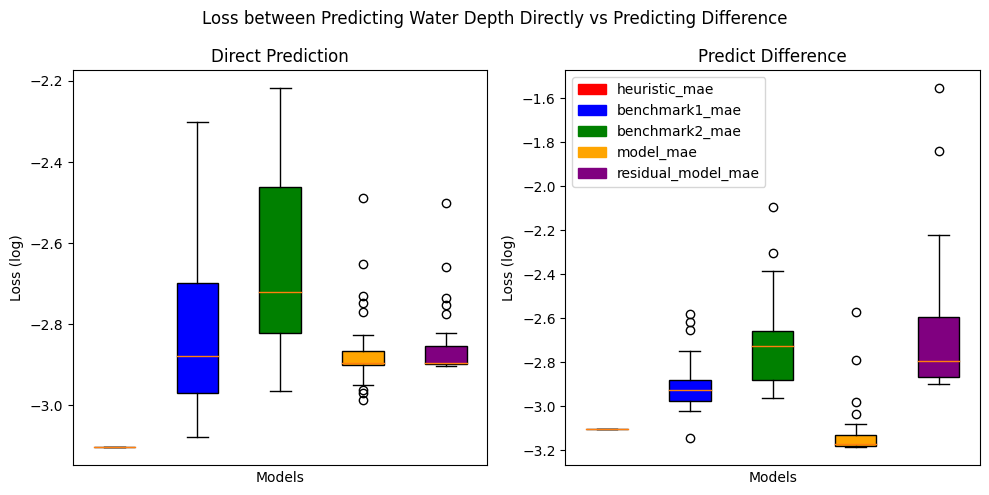
\includegraphics[width=0.8\linewidth, height=0.3\textheight]{Figures/Results/Diff_Complexity_Lr_Epochs/Predicting_Diff/box_dif_v_no_diff}
	\caption[Predicting water depth difference vs predicting water depth directly]{Loss for predicting water depth directly vs predicting the difference in water depth}
	\label{fig:diffvsnodiff}
\end{figure}

Fig \ref{fig:diffvsnodiff} shows that models trained to predict water depth directly have much more variability. Loss  for predicting a single time step has more outliers and performs worse on average than predicting the difference in water depth. However, it seems that recurrent time step prediction performs better. Only models that predict difference in water depth over a single time step perform better than the heuristic. Based on these results, further evaluation is only based on predicting difference in water depth.

\subsubsection*{Model Complexity, Predicting Difference in Water Depth}
Fig. \ref{fig:depthwise-complexity} shows the loss of different model complexities across epochs and learning rates. The shallow DepthwiseCNN model seems to show the best results. All model complexities out-perform the heuristic. Unfortunately, whilst generating data and deciding which models to do further testing on, only the best models were considered. In this case, the best performing model was a medium complexity model (see 5th row of Table \ref{tab:best_ss}). So further work was done on the medium complexity model. Further testing should be done on a simpler model \footnote{see section \ref{Extra} for a small further look into a simpler model and it the benefits it showed}, especially where the recurrent (and most useful) loss is concerned. 
\begin{figure}[tbph]
	\centering
	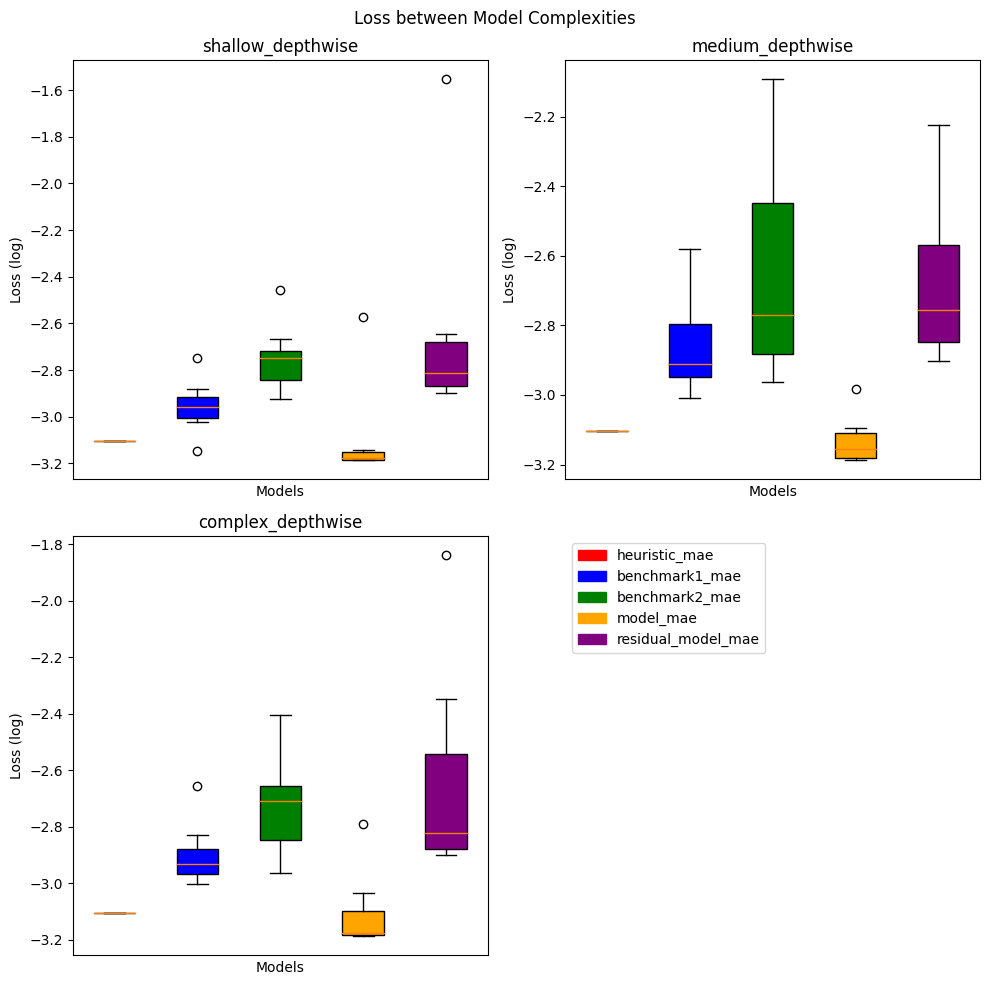
\includegraphics[width=0.7\linewidth, height=0.4\textheight]{Figures/Results/Diff_Complexity_Lr_Epochs/Complexity/Box_model_complexity}
	\caption[Loss Depending on Model Complexity for DepthwiseCNN]{Loss for different model complexities that predict water difference}
	\label{fig:depthwise-complexity}
\end{figure}


\subsubsection*{Epochs and Learning Rate for Medium Complexity DepthwiseCNN}
Fig \ref{fig:epochs} shows the model loss for the medium complexity DepthwiseCNN. This is across a variety of learning rates, which are shown in Table \ref{tab:lr}. There was very little difference between the epochs. A reason for this might be due to the stop loss callback option used during training. Overall, across all testing, models struggled to learn anything. A reason for this may be due to being trapped in local minima from the start. If the model was predicting no change, the loss was very low and even outperformed the heuristic. Fig \ref{fig:egloss-epochs} shows an example loss across all models (benchmark and DepthwiseCNN model). Where m is the model, b1, is benchmark 1 and b2 is benchmark 2. The reason for the large difference in loss is due to the type of loss functions employed. The benchmark models were always trained using standard MAE and default learning rate of 1e-3. The custom loss functions used for training the model of interest always increased the loss by 1000 times. The motivation for this was it would be easier to for the model to learn from a larger loss than a tiny loss.

\begin{figure}[tbph]
	\centering
	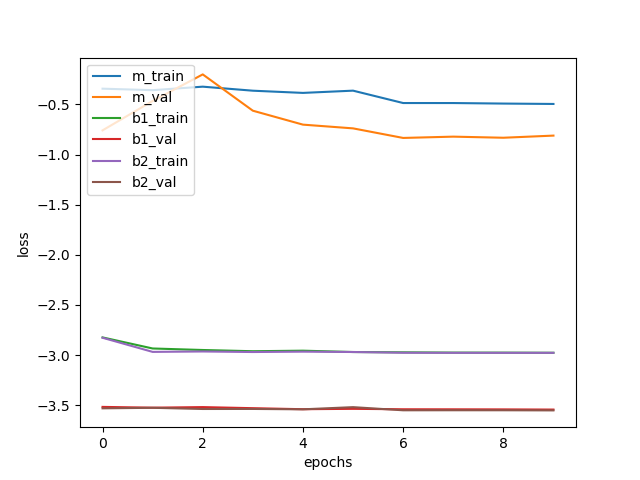
\includegraphics[width=0.9\linewidth, height=0.3\textheight]{Figures/Results/Diff_Complexity_Lr_Epochs/Epochs_Lr/medium_depthwise_diff_train_2_custom_mae_weighted_2e-3_more_epochs_norm_independant_292_training}
	\caption[Example Loss for Medium depthwise model and benchmarks]{Example training loss for medium depthwise model and benchmarks}
	\label{fig:egloss-epochs}
\end{figure}


\begin{figure}[tbph]
	\centering
	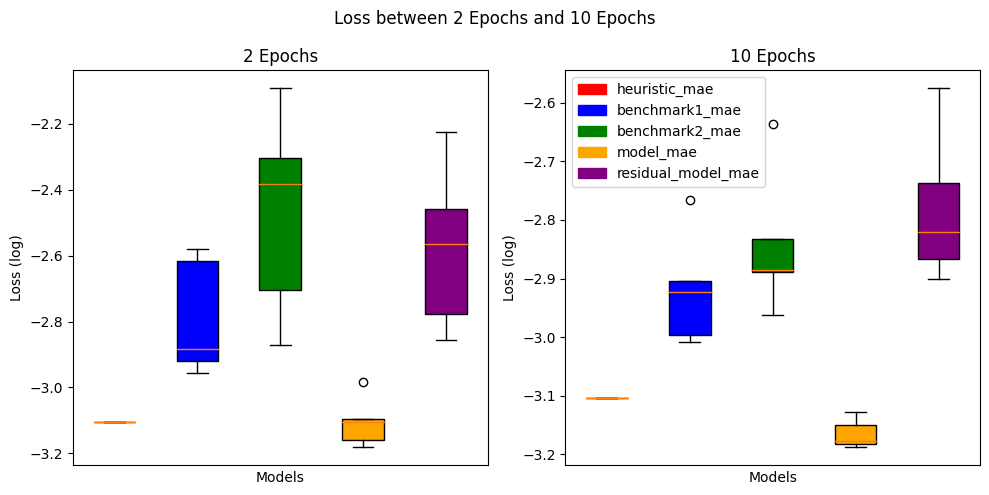
\includegraphics[width=0.8\linewidth, height=0.3\textheight]{Figures/Results/Diff_Complexity_Lr_Epochs/Epochs_Lr/Box_epochs}
	\caption[Loss between two different Epochs]{Loss for medium complexity DepthwiseCNN model over two different epochs}
	\label{fig:epochs}
\end{figure}

From Table \ref{tab:lr}, the different learning rates had little effect on model performance. All learning rates performed better than the heuristic for medium complexity models. However, there did seem to be an effect on recurrent time step predictions. A learning rate of 1e-4 seemed to show the most promise, at least for recurrent time step predictions so this is what we use moving  forward, unless otherwise specified.
\begin{table}[htbp]
	\centering
	\caption{Final losses for different learning rate with Medium Complexity}
	\label{tab:lr}
	\begin{tabular}{p{2cm}ccccc}
		\toprule
		Name &  H &  BM1 &  BM2 &  Model &  Recurrent \\
		\midrule
		1e-3 &       0.000787 &        0.001194 &        0.001092 &   0.000665 &            0.001510 \\
		2e-3 &       0.000787 &        0.001010 &        0.001302 &   0.000658 &            0.001360 \\
		1e-4 &       0.000787 &        0.001714 &        0.002307 &   0.000648 &            0.001254 \\
		1e-2 &       0.000787 &        0.001246 &        0.001473 &   0.000744 &            0.002659 \\
		5e-4 &       0.000787 &        0.000982 &        0.001290 &   0.000707 &            0.001836 \\
		\bottomrule
	\end{tabular}
\end{table}

\subsubsection*{Optimal Weights for MAE}
Table \ref{tab:weights} shows the loss for different weights for the Manual MAE loss function. (see Fig. \ref{fig:MAE-weights-init} for a visual representation). 
\begin{figure}[tbph]
	\centering
	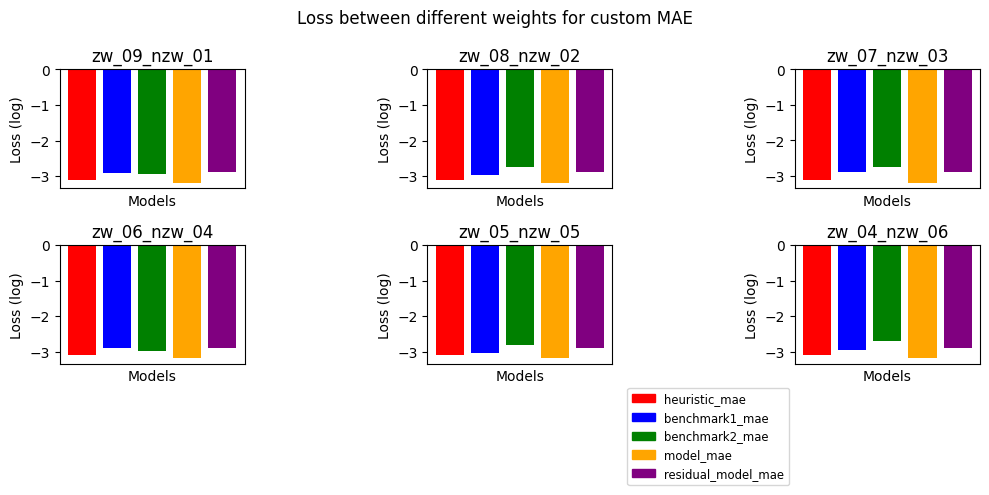
\includegraphics[width=0.9\linewidth, height=0.5\textheight]{Figures/Results/Shuffle_Weights/weights/weights}
	\caption[Loss for Different Weights of MAE]{Loss for Different Weights of MAE}
	\label{fig:MAE-weights-init}
\end{figure}

\begin{table}[htbp]
	\centering
	\caption{The loss for different weightings in the MAE manuel loss function}
	\label{tab:weights}
	\begin{tabular}{p{2cm}ccccc}
		\toprule
		Name &  H &  BM1 &  BM2 &  Model &  Recurrent \\
		\midrule
		09|01 &       0.000787 &        0.001204 &        0.001137 &   0.000655 &            0.001322 \\
		08|02 &       0.000787 &        0.001042 &        0.001830 &   0.000654 &            0.001335 \\
		07|03 &       0.000787 &        0.001276 &        0.001845 &   0.000649 &            0.001267 \\
		06|04 &       0.000787 &        0.001248 &        0.001051 &   0.000652 &            0.001302 \\
		05|05 &       0.000787 &        0.000894 &        0.001517 &   0.000649 &            0.001260 \\
		04|06 &       0.000787 &        0.001127 &        0.002029 &   0.000649 &            0.001263 \\
		\bottomrule
	\end{tabular}
\end{table}
Where the name indicates zero weight and non zero weight respectively. (eg. zero weight of 0.9 and non zero weight of 0.1, i.e. 0.9|0.1). \\

Since the Manual MAE loss function performed the best. The correct weight ratio was searched for. In Table \ref{tab:weights}, we see no meaningful difference (at most 0.000006 difference between weights.) This is a surprising result but as can be seen in Fig \ref{fig:egloss-epochs} models struggle to learn in general. Manual MAE with weighting of 0.5 | 0.5 was used for the rest of the evaluations unless otherwise specified.

\subsubsection*{Shuffling the Data}]
Table \ref{tab:suffle} shows the results of shuffling the data using the function 'train \_ test \_ split()' from the python library sklearn with kwarg** shuffle=True. There was no meaningful difference between shuffling the data or not.
\begin{table}[h]
	\centering
	\caption{The loss for shuffled or not shuffled}
	\label{tab:suffle}
	\begin{tabular}{p{2cm}ccccc}
		\toprule
		Name &  H &  BM1 &  BM2 &  Model &  Recurrent \\
		\midrule
		Shuffled &       0.000787 &        0.002165 &        0.001247 &   0.000648 &            0.001255 \\
		Sequential &       0.000787 &        0.001578 &        0.001307 &   0.000649 &            0.001263 \\
		\bottomrule
	\end{tabular}
\end{table}

\section{Additional Features}

Fig \ref{fig:norm-rain-mask-init} shows the loss of models between the different feature datasets. From this plot it is clear that the original, independently normalized dataset shows the most constant and lowest losses across the board. So this is the dataset that will be considered for further evaluation. The motivation added rainfall directly to the water depth, is this is how the CADDIE model works. Unfortunately, due to the fact there are so little features anyway, the  model was not able to correctly learn with this data. Although the model still outperformed the heuristic. Then the mask dataset is tested. The motivation is again because of the CADDIE model. Areas outside the catchment are considered run-off and some masked areas might make it into the training dataset. It would be hard for the model to differentiate the zero padding (which is there to preserve the shape of the input) from a masked area that should be run-off. 
\begin{figure}[tbph]
	\centering
	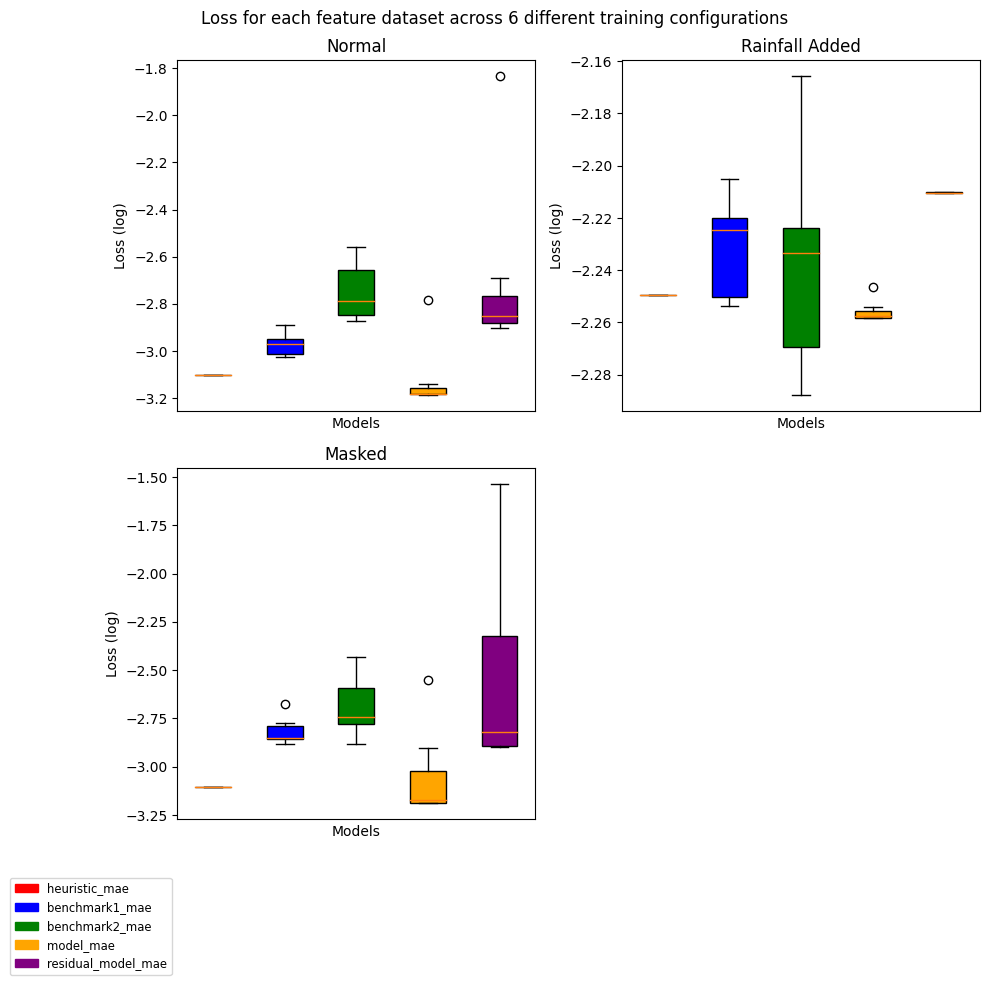
\includegraphics[width=0.7\linewidth, height=0.5\textheight]{Figures/Results/feature_manip/feature_manip_across_lr}
	\caption[Loss For Three different Datasets With Different Features]{Loss for Three different Datasets with Different Features across varying training configurations}
	\label{fig:norm-rain-mask-init}
\end{figure}

\begin{table}[htbp]
	\centering
	\caption{Six training configurations testing two different weights for MAE Manuel and three lr across the original, normalized dataset}
	\label{tab:weighte_lr}
	\begin{tabular}{p{2cm}ccccc}
		\toprule
		Name &  H &  BM1 &  BM2 &  Model &  Recurrent \\
		\midrule
		w11 &       0.000787 &        0.001163 &        0.001336 &   0.000669 &            0.001453 \\
		w12 &       0.000787 &        0.000958 &        0.001636 &   0.000726 &            0.002032 \\
		w13 &       0.000787 &        0.001284 &        0.001447 &   0.000658 &            0.001350 \\
		w21 &       0.000787 &        0.001067 &        0.002772 &   0.001642 &            0.014677 \\
		w22 &       0.000787 &        0.000942 &        0.002398 &   0.000657 &            0.001403 \\
		w23 &       0.000787 &        0.000990 &        0.002026 &   0.000648 &            0.001255 \\
		\bottomrule
	\end{tabular}
\end{table}

Where the first number indicates the weight ratio,
\begin{enumerate}
	\item 0.5|0.5
	\item  0.2|0.8
\end{enumerate}

And the second number indicates the learning rate,
\begin{enumerate}
	\item  1e-2
	\item  1e-3
	\item  1e-4
\end{enumerate}
For example [w11] from Table \ref{tab:weighte_lr} is the weight ratio of 0.5 zero weight and 0.5 non zero weight, with a learning rate of 1e-2. Here we see that such a high learning rate negatively impacts models and reaffirms that the weights had little impact except in the case of [w21] which performed much worst than the rest in terms of loss. One "success" was for a different weighting scheme but was not able to be reproduced  can be seen in Fig \ref{fig:random-success}. The it was trained on the original, independently normalized dataset, with a learning rate of 1e-4, using the Manual MAE loss function with weights 0.1 | 0.9.

\begin{figure}[tbph]
	\centering
	\includegraphics[width=0.8\linewidth, height=0.3\textheight]{"Figures/Results/feature_manip/medium_depthwise_diff_train_4_custom_mae_weighted_7_20 epochs_norm_independant_normal_292_random_cell_residual"}
	\caption[Medium depthwise model random cell residual time step predictions]{Medium depthwise model random cell residual time step predictions}
	\label{fig:random-success}
\end{figure}

This figure shows the ability of the model to learn a non-linear recurrent  prediction, which was not seen prior, and provides some glimmer of hope that a DL model is capable of learning flood modeling.


\section{Inception Inspired Model}
In this section, column names are w1, w2, w3, They represent the following training regime,
\begin{enumerate}
	\item[w1] 20 Epochs, learning rate of 1e-2, Manual MAE with zero weight 0,2 and non zero weight of 0,8
	\item[w2] 20 Epochs, learning rate of 1e-3, Manual MAE with zero weight 0,2 and non zero weight of 0,8
	\item[w3] 20 Epochs, learning rate of 1e-3, Manual MAE with zero weight 0,1 and non zero weight of 0,9
\end{enumerate}

The motivation for using this model is it's ability to generate it's own feature maps using a variety techniques and then concatenating the results, which is then fed into into another sequential layer. Overall the results are quite similar to the DepthwiseCNN models but did perform, albeit, slightly better.

\subsubsection*{Training Across Different Feature Datasets}
Fig. \ref{fig:incep-normaldset}, \ref{fig:incep-rfdset}, \ref{fig:incep-maskdset} are the plots showing the losses of two different model complexities, simple and medium, across varying learning rates and weights for the Manual MAE (see above). The models performed the best on the independently normalized dataset, as with the DepthwiseCNN model from the previous section. However, it seems that the masked dataset showed  less variability for recurrent predictions. Fig. \ref{fig:eg-simpincep} shows that the simple complexity Inception Inspired model also manages to learn something for recurrent predictions.


\begin{figure}[tbph]
	\centering
	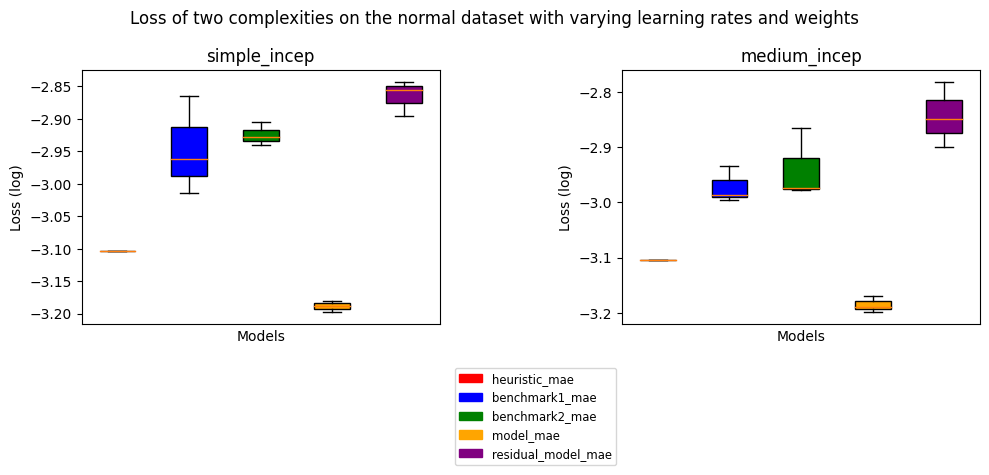
\includegraphics[width=0.8\linewidth, height=0.3\textheight]{Figures/Results/Inception_model/normal_dataset}
	\caption[Loss for Inception Inspired model for two different complexities on the normal dataset]{Loss for Inception Inspired model for two different complexities on the normal dataset}
	\label{fig:incep-normaldset}
\end{figure}


\begin{figure}[tbph]
	\centering
	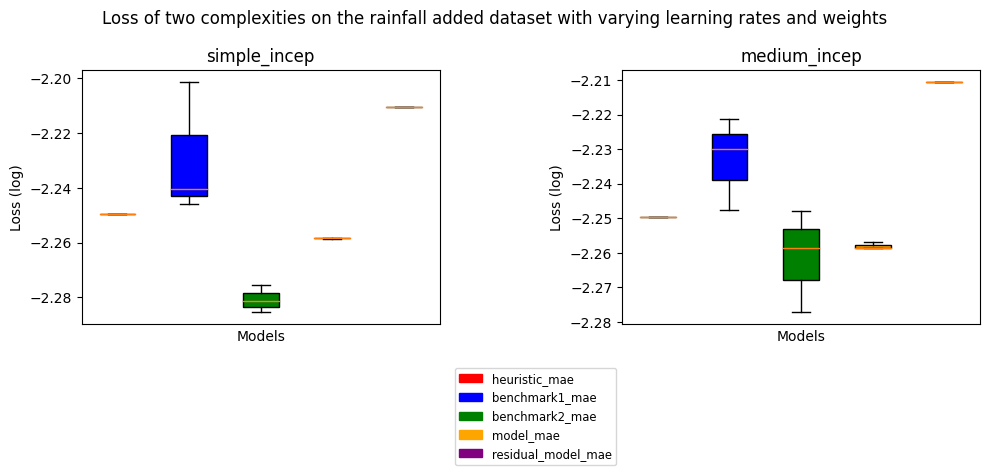
\includegraphics[width=0.8\linewidth, height=0.3\textheight]{Figures/Results/Inception_model/rainfall_dataset}
	\caption[Loss for Inception Inspired model for two different complexities on the added rainfall dataset]{Loss for Inception Inspired model for two different complexities on the added rainfall dataset}
	\label{fig:incep-rfdset}
\end{figure}

\begin{figure}[tbph]
	\centering
	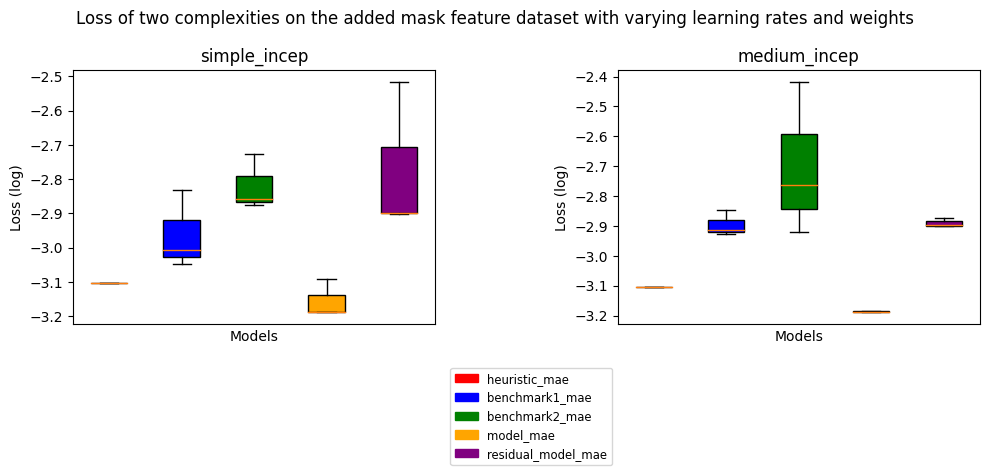
\includegraphics[width=0.8\linewidth, height=0.3\textheight]{Figures/Results/Inception_model/mask_dataset}
	\caption[Loss for Inception Inspired model for two different complexities on the added mask dataset]{Loss for Inception Inspired model for two different complexities on the added masked dataset}
	\label{fig:incep-maskdset}
\end{figure}

\begin{figure}[tbph]
	\centering
	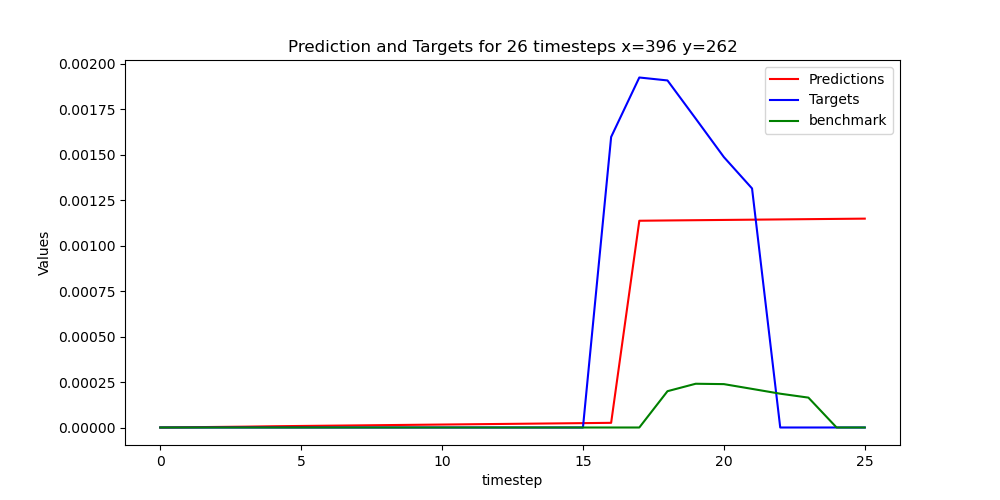
\includegraphics[width=0.8\linewidth, height=0.3\textheight]{Figures/Results/Inception_model/simple_incep_train_5_custom_mae_weighted_10_norm_independant_normal_292_random_cell_residual}
	\caption[Simple Inception Inspired model on original independently normed dataset]{Simple Inception Inspired model on original independently normed dataset for a random cell predicting recurrently}
	\label{fig:eg-simpincep}
\end{figure}


\subsubsection*{Simple model}
Table \ref{tab:simple_normal} shows that the different training regimes don't have meaningful impact on results. An example loss can be seen in Fig \ref{fig:simple-incep-loss}, where the results from training are very reminiscent of the DepthwiseCNN architecture. 
\begin{table}[htbp]
	\centering
	\caption{Three training configurations on the normal dataset for simple inception based model}
	\label{tab:simple_normal}
	\begin{tabular}{p{2cm}ccccc}
		\toprule
		Name &  H &  BM1 &  BM2 &  Model &  Recurrent \\
		\midrule
		w1 &       0.000787 &        0.000966 &        0.001179 &   0.000661 &            0.001437 \\
		w2 &       0.000787 &        0.001093 &        0.001247 &   0.000648 &            0.001272 \\
		w3 &       0.000787 &        0.001366 &        0.001146 &   0.000634 &            0.001396 \\
		\bottomrule
	\end{tabular}
\end{table}


\begin{figure}[tbph]
	\centering
	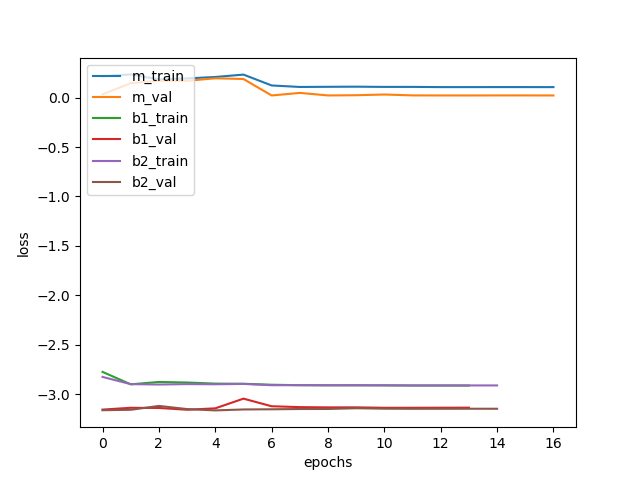
\includegraphics[width=0.8\linewidth, height=0.3\textheight]{Figures/Results/Inception_model/simple_incep_train_5_custom_mae_weighted_8_norm_independant_rf_added_292_training}
	\caption[Loss during training of simple inception inspired model versus benchmark models]{Loss during training of simple inception inspired model versus benchmark models}
	\label{fig:simple-incep-loss}
\end{figure}

In Table \ref{tab:simple_rf} we see that the model has the worst overall loss when comparing against the other feature datasets.
\begin{table}[htbp]
	\centering
	\caption{Three training configurations on the rainfall added dataset for simple inception based model}
	\label{tab:simple_rf}
	\begin{tabular}{p{2cm}ccccc}
		\toprule
		Name &  H &  BM1 &  BM2 &  Model &  Recurrent \\
		\midrule
		w1 &       0.005629 &        0.005676 &        0.005305 &   0.005517 &            0.006159 \\
		w2 &       0.005629 &        0.006293 &        0.005231 &   0.005514 &            0.006159 \\
		w3 &       0.005629 &        0.005750 &        0.005183 &   0.005519 &            0.006159 \\
		\bottomrule
	\end{tabular}
\end{table}

\begin{table}[htbp]
	\centering
	\caption{Three training configurations on the mask added dataset for simple inception based model}
	\label{tab:simple_mask}
	\begin{tabular}{p{2cm}ccccc}
		\toprule
		Name &  H &  BM1 &  BM2 &  Model &  Recurrent \\
		\midrule
		w1 &       0.000787 &        0.000986 &        0.001333 &   0.000811 &            0.003052 \\
		w2 &       0.000787 &        0.001469 &        0.001390 &   0.000648 &            0.001262 \\
		w3 &       0.000787 &        0.000897 &        0.001878 &   0.000648 &            0.001253 \\
		\bottomrule
	\end{tabular}
\end{table}


\subsubsection*{Medium Model}
The Medium complexity model increases parameter count dramatically. The results are shown below.
\begin{table}[htbp]
	\centering
	\caption{Three training configurations on the normal dataset for medium inception based model}
	\label{tab:medium_normal}
	\begin{tabular}{p{2cm}ccccc}
		\toprule
		Name &  H &  BM1 &  BM2 &  Model &  Recurrent \\
		\midrule
		w1 &       0.000787 &        0.001032 &        0.001054 &   0.000676 &            0.001655 \\
		w2 &       0.000787 &        0.001166 &        0.001064 &   0.000632 &            0.001418 \\
		w3 &       0.000787 &        0.001011 &        0.001362 &   0.000648 &            0.001258 \\
		\bottomrule
	\end{tabular}
\end{table}

\begin{table}[htbp]
	\centering
	\caption{Three training configurations on the rainfall added dataset for medium inception based model}
	\label{tab:medium_rf}
	\begin{tabular}{p{2cm}ccccc}
		\toprule
		Name &  H &  BM1 &  BM2 &  Model &  Recurrent \\
		\midrule
		w1 &       0.005629 &        0.005655 &        0.005513 &   0.005534 &            0.006159 \\
		w2 &       0.005629 &        0.006006 &        0.005282 &   0.005514 &            0.006160 \\
		w3 &       0.005629 &        0.005888 &        0.005650 &   0.005514 &            0.006160 \\
		\bottomrule
	\end{tabular}
\end{table}

\begin{table}[htbp]
	\centering
	\caption{Three training configurations on the mask added dataset for medium inception based model}
	\label{tab:medium_mask}
	\begin{tabular}{p{2cm}ccccc}
		\toprule
		Name &  H &  BM1 &  BM2 &  Model &  Recurrent \\
		\midrule
		w1 &       0.000787 &        0.001427 &        0.003831 &   0.000654 &            0.001342 \\
		w2 &       0.000787 &        0.001183 &        0.001719 &   0.000647 &            0.001254 \\
		w3 &       0.000787 &        0.001222 &        0.001197 &   0.000650 &            0.001267 \\
		\bottomrule
	\end{tabular}
\end{table}

From Tables \ref{tab:medium_normal}, \ref{tab:medium_rf}, \ref{tab:medium_mask}, The results for the masked and normal datasets are similar but best results are still seen in the original independent dataset. Although the medium complexity Inception Inspired model outperforms the simple version, the increased parameter count and time needed to train also needs to be considered in future evaluations. In the below section, results across all training of all models are compared. \\

\section{Final Results}
\begin{table}[htbp]
	\centering
	\caption{The Top Five Models Across all Training SS}
	\label{tab:best_ss}
	\begin{tabular}{p{2cm}ccccc}
		\toprule
		Name &  H &  BM1 &  BM2 &  Model &  Recurrent \\
		\midrule
		1 &       0.000787 &        0.001166 &        0.001064 &   0.000632 &            0.001418 \\
		2 &       0.000787 &        0.001366 &        0.001146 &   0.000634 &            0.001396 \\
		3 &       0.000787 &        0.001183 &        0.001719 &   0.000647 &            0.001254 \\
		4 &       0.000787 &        0.001011 &        0.001362 &   0.000648 &            0.001258 \\
		5 &       0.000787 &        0.002165 &        0.001247 &   0.000648 &            0.001255 \\
		\bottomrule
	\end{tabular}
\end{table}
Table \ref{tab:best_ss} shows the top performing models for predicting a single time step (SS) ahead, overall across all testing. The Name column has the following keys,
\begin{enumerate}
	\item Medium Complexity Inception Inspired Model on the normalized dataset with the original three features. Trained with 20 Epochs, a learning rate of 1e-3, Manual MAE loss with zero weighting of 0,2 and non zero weighting 0,8.
	\item Simple Complexity Inception Inspired Model on the normalized dataset. Trained with 20 Epochs, a learning rate of 1e-3, Manual MAE loss with zero weighting of 0,1 and non zero weighting 0,9.
	\item Medium Complexity Inception Inspired Model on the normalized dataset with an additional mask feature. Trained with 20 Epochs, a learning rate of 1e-3, Manual MAE loss with zero weighting of 0,2 and non zero weighting 0,8.
	\item Medium Complexity Inception Inspired Model on the normalized dataset with the original three features. Trained with 20 Epochs, a learning rate of 1e-3, Manual MAE loss with zero weighting of 0,1 and non zero weighting 0,9.
	\item Medium complexity DepthwiseCNN model on the normalized dataset with original features. Trained with 8 Epochs,a learning rate of 1e-4, Manual MAE loss with zero weighting of 0,5 and non zero weighting of 0,5.
\end{enumerate}

\begin{table}[htbp]
	\centering
	\caption{The Top Five Models Across all Training For Recurrent Steps}
	\label{tab:best_r}
	\begin{tabular}{p{2cm}ccccc}
		\toprule
		Name &  H &  BM1 &  BM2 &  Model &  Recurrent \\
		\midrule
		1 &       0.000787 &        0.001502 &        0.001632 &   0.001253 &            0.001253 \\
		2 &       0.000787 &        0.000897 &        0.001878 &   0.000648 &            0.001253 \\
		3 &       0.000787 &        0.001183 &        0.001719 &   0.000647 &            0.001254 \\
		4 &       0.000787 &        0.002816 &        0.003378 &   0.001254 &            0.001254 \\
		5 &       0.000787 &        0.001714 &        0.002307 &   0.000648 &            0.001254 \\
		\bottomrule
	\end{tabular}
\end{table}
Table \ref{tab:best_r} shows the top five models based on recurrent water depth prediction across all training. The name column has the following key-value pairs,
\begin{enumerate}
	\item Medium Complexity DepthwiseCNN model predicting water depth directly. Trained on the normalized dataset with 10 epochs, a learning rate of 1e-4. 
	\item Simple Complexity Inception Inspired model the normalized dataset with the added mask feature. Trained with 20 Epochs, a learning rate of 1e-3, Manual MAE loss with zero weighting of 0,1 and non zero weighting 0,9.
	\item Medium Complexity Inception Inspired Model on the normalized dataset with the  added mask feature, predicting difference in water depth. Trained with 20 Epochs, a learning rate of 1e-3, Manual MAE loss with zero weighting of 0,2 and non zero weighting 0,8.
	\item Medium Complexity DepthwiseCNN model predicting water depth directly. Trained on the normalized dataset with 2 epochs, a learning rate of 1e-4.
	\item Medium Complexity DepthwiseCNN model predicting the difference in  water depth. Trained on the normalized dataset with 10 epochs, a learning rate of 1e-4.
\end{enumerate}

\begin{table}[htbp]
	\centering
	\caption{The Worst Five Models Across all Training For SS}
	\label{tab:worstss}
	\begin{tabular}{p{2cm}ccccc}
		\toprule
		Name &  H &  BM1 &  BM2 &  Model &  Recurrent \\
		\midrule
		1 &       0.002279 &       81.628900 &      106.629910 &  44.619150 &          648.459210 \\
		2 &       0.002279 &       78.769480 &      111.990715 &  32.265385 &          379.157455 \\
		3 &       0.002551 &       14.399827 &       25.591928 &  16.135822 &          187.824300 \\
		4 &       0.002551 &       21.657652 &       24.267190 &   8.066945 &          101.351124 \\
		5 &       0.002551 &       18.857510 &       27.992000 &   5.856058 &           83.558502 \\
		\bottomrule
	\end{tabular}

\end{table}
Table \ref{tab:worstss} shows the worst five performing models for predicting a single time step (SS) ahead, overall across all testing. The Name column has the following keys,
\begin{enumerate}
	\item Inital Depthwise Model using classic MSE on the DEM 26 dataset where everything was min max normalized using the DEM. Trained using 2 Epochs, default learning rate of 1e-3.
	\item Inital Depthwise Model using Manual MSE on the DEM 26 dataset where everything was min max normalized using the DEM. Trained using 2 Epochs, default learning rate of 1e-3. zero weight of 0.8 and non zero weight of 0.2.
	\item Inital Depthwise Model using classic MSE on the DEM 819 dataset where everything was min max normalized using the DEM. Trained using 2 Epochs, default learning rate of 1e-3.
	\item Inital Depthwise Model using  Manual MSE on the DEM 819 dataset where everything was min max normalized using the DEM. Trained using 2 Epochs, default learning rate of 1e-3. zero weight of 0.8 and non zero weight of 0.2.
	\item Inital Depthwise Model using  auto MSE on the DEM 819 dataset where everything was min max normalized using the DEM. Trained using 2 Epochs, default learning rate of 1e-3.
\end{enumerate}


\begin{table}[htbp]
	\centering
	\caption{The Worst Five Models Across all Training For Recurrent Steps}
	\label{tab:worstr}
	\begin{tabular}{p{2cm}ccccc}
		\toprule
		Name &  H &  BM1 &  BM2 &  Model &  Recurrent \\
		\midrule
		1 &       0.002279 &       81.628900 &      106.629910 &  44.619150 &          648.459210 \\
		2 &       0.002279 &       78.769480 &      111.990715 &  32.265385 &          379.157455 \\
		3 &       0.002551 &       14.399827 &       25.591928 &  16.135822 &          187.824300 \\
		4 &       0.002440 &        4.586013 &       38.804940 &   4.971159 &          164.466783 \\
		5 &       0.001346 &        0.001753 &        0.002407 &   0.002654 &          119.582068 \\
		\bottomrule
	\end{tabular}
\end{table}

Table \ref{tab:worstr} shows the worst five performing models for predicting recurrent time steps ahead, overall across all testing. The Name column has the following keys,
\begin{enumerate}
	\item Inital Depthwise Model using classic MSE on the DEM 26 dataset where everything was min max normalized using the DEM. Trained using 2 Epochs, default learning rate of 1e-3.
	\item Inital Depthwise Model using Manual MSE on the DEM 26 dataset where everything was min max normalized using the DEM. Trained using 2 Epochs, default learning rate of 1e-3. zero weight of 0.8 and non zero weight of 0.2.
	\item Inital Depthwise Model using classic MSE on the DEM 819 dataset where everything was min max normalized using the DEM. Trained using 2 Epochs, default learning rate of 1e-3.
	\item Inital Depthwise Model using  auto MAE on the DEM 292 dataset where everything was min max normalized using the DEM. Trained using 2 Epochs, default learning rate of 1e-3.
	\item Inital Depthwise Model using  auto MSE on the DEM 819 dataset where features are normalized independently. Trained using 2 Epochs, default learning rate of 1e-3.
\end{enumerate}

The following plots where created after all initial testing to try and reproduce the models. Fig. \ref{fig:BRMR} shows the water depths of the true values, heuristic model output, and deep learning model predictions of a random cell in the test set using a recurrent time step method prediction. The model used was the best performing model for a single time step prediction.  (see Table. \ref{tab:best_r}). Fig. \ref{fig:BRMS} shows the same plot but predicting a single time step ahead. Fig. \ref{fig:BSMR} and \ref{fig:BSMS} are the plots respectively but using the best single time step model (see Table. \ref{tab:best_ss}).

\begin{figure}[tbph]
	\centering
	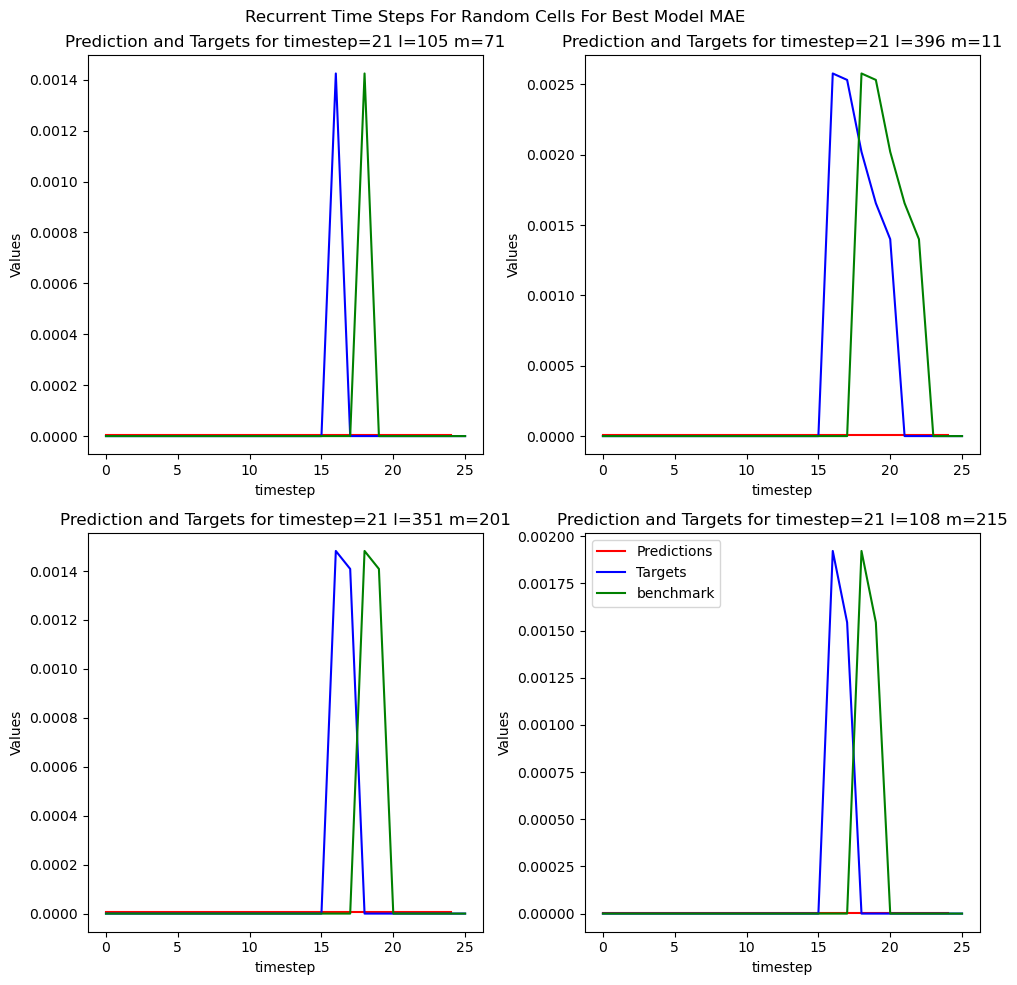
\includegraphics[width=0.8\linewidth, height=0.3\textheight]{Figures/Results/Final_Results/Best_Model_recurrentMAE_recurrent_random_cell}
	\caption[Best Recurrent MAE random cell over time]{Water Depth Predictions recurrently over the test set timesteps}
	\label{fig:BRMR}
\end{figure}



\begin{figure}[tbph]
	\centering
	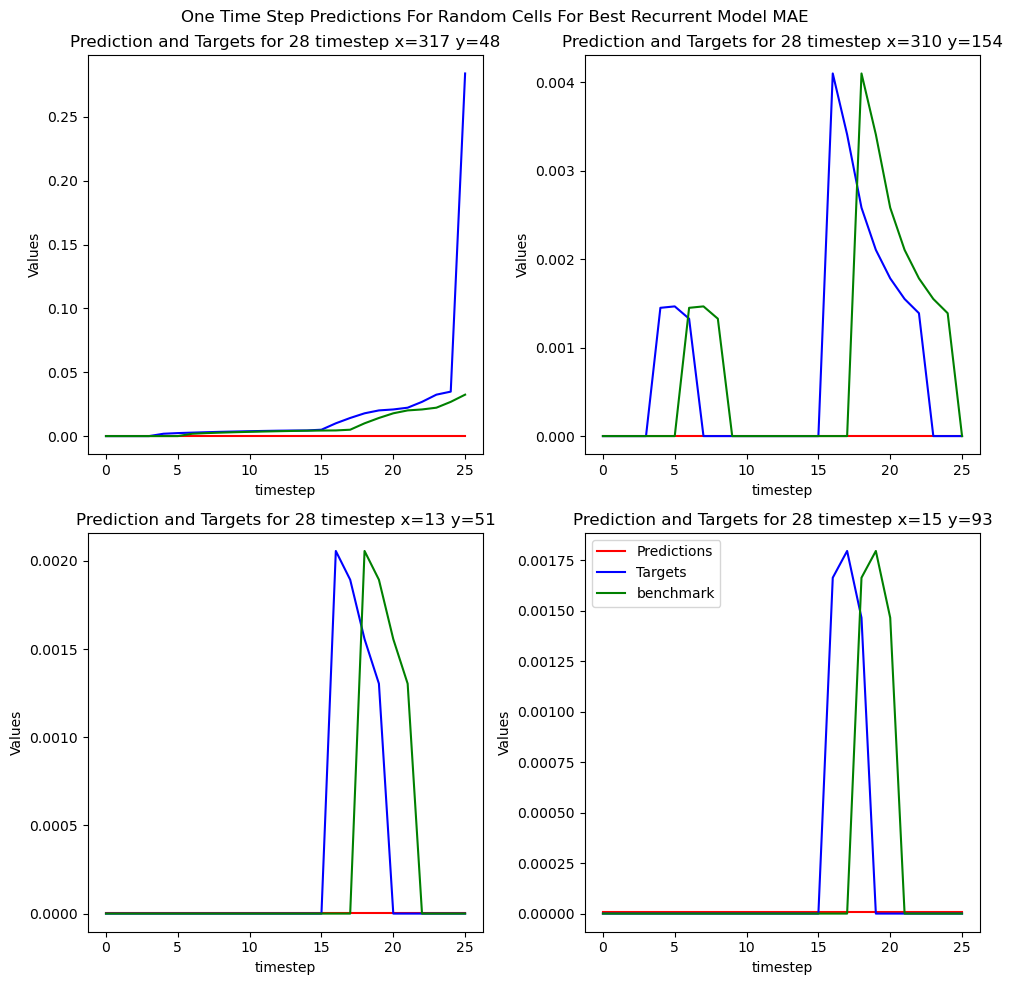
\includegraphics[width=0.8\linewidth, height=0.3\textheight]{Figures/Results/Final_Results/Best_Model_recurrentMAE_SS_random_cell}
	\caption[Best Recurrent Loss on single time step predictions over test set]{Best Recurrent Loss on single time step predictions over test set}
	\label{fig:BRMS}
\end{figure}


\begin{figure}[tbph]
	\centering
	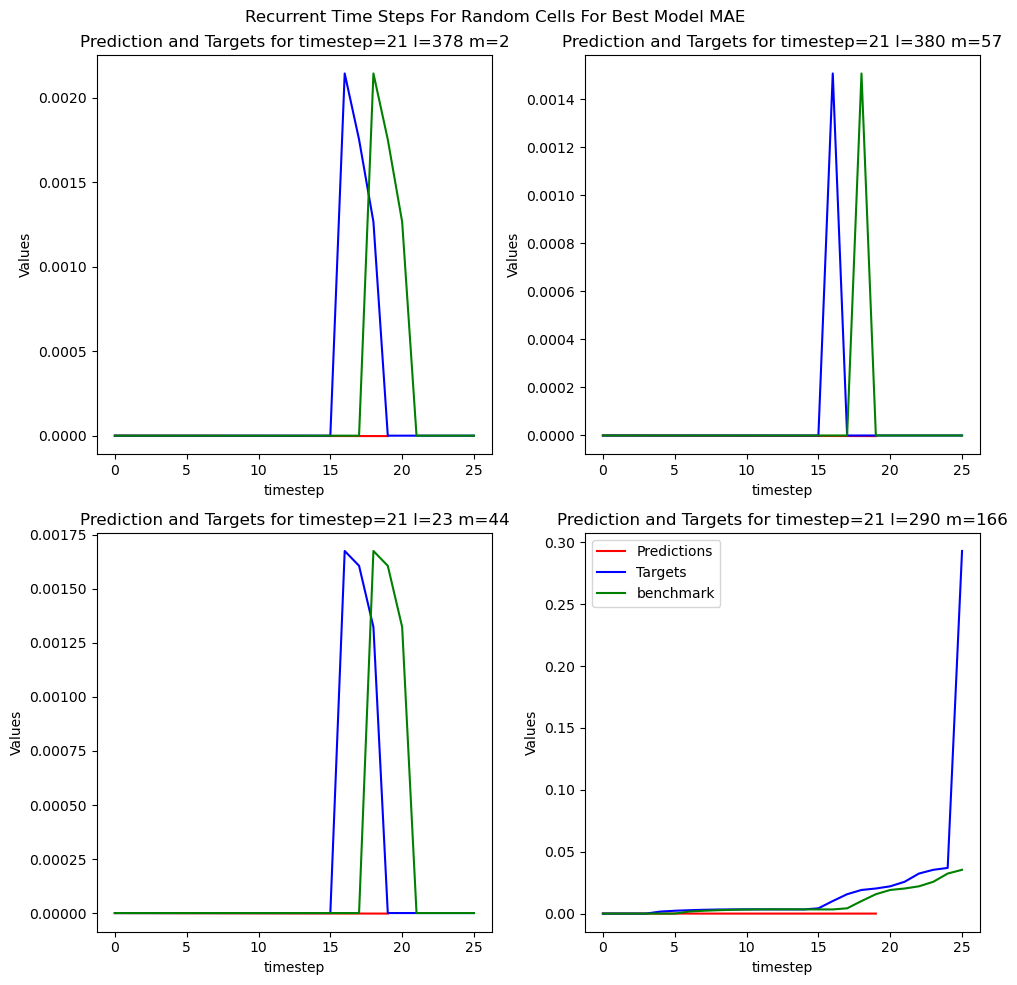
\includegraphics[width=0.8\linewidth, height=0.3\textheight]{Figures/Results/Final_Results/Best_Model_SS_recurrent_random_cell}
	\caption[Best single step model on test set predicting water depth for recurrent time steps]{Best single step model on test set predicting water depth for recurrent time steps}
	\label{fig:BSMR}
\end{figure}

\begin{figure}[tbph]
	\centering
	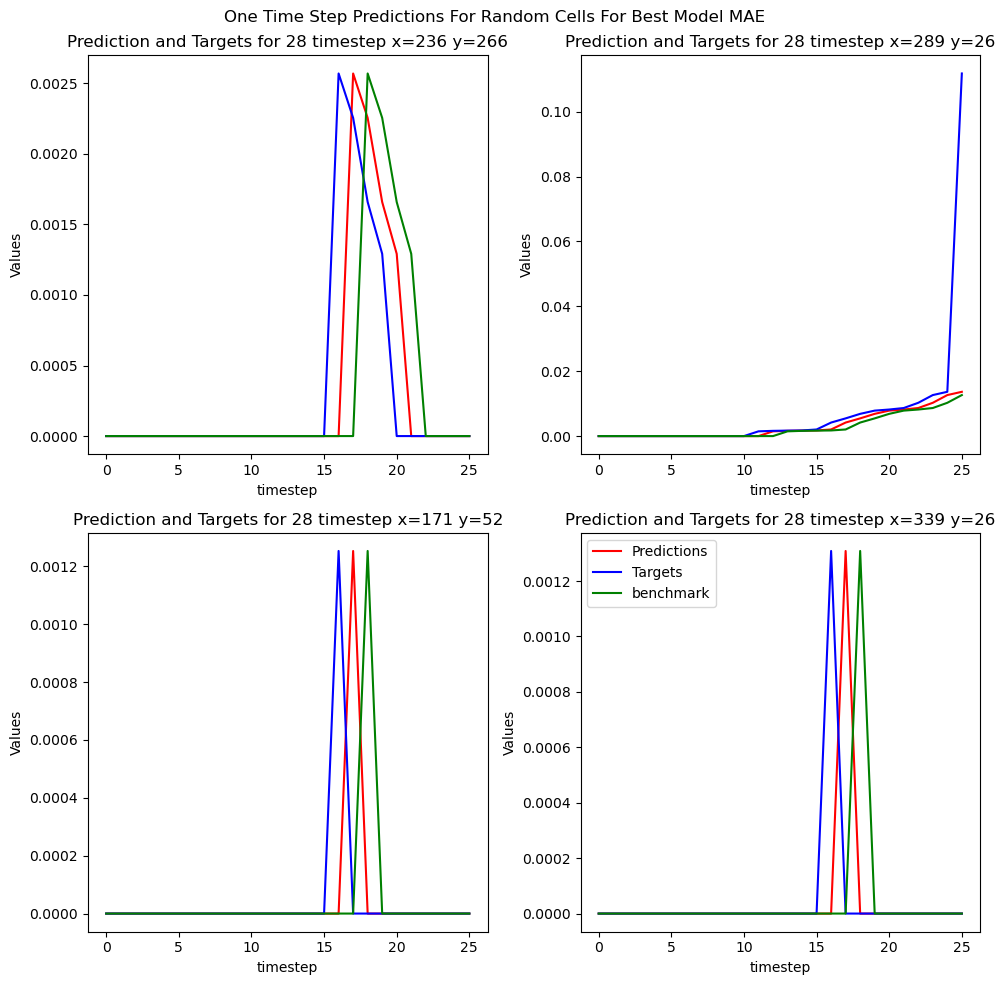
\includegraphics[width=0.8\linewidth, height=0.3\textheight]{Figures/Results/Final_Results/Best_Model_SS_SS_random_cell}
	\caption[Best single time step model on predicting water depth for a single time step]{Best single time step model on predicting water depth for a single time step}
	\label{fig:BSMS}
\end{figure}

Fig. \ref{fig:SpatialTrue} shows the spatial evolution of water depth on the test set and is used for comparison. Fig. \ref{fig:BMS-spatial} shows the best model from Table \ref{tab:best_ss} and its spatial evolution of water depth over the test set. Fig. \ref{fig:adjusted-spatial} shows the spatial evolution of water depth on the test set using recurrent predictions. All other models predicted 0. This model is a slightly adjusted model, trained on lower epochs (2) and adjusting MAE weighting to 0.5 | 0.5. Fig. \ref{fig:adjusted-recurrent-rc} shows the recurrent preditions of a collection of random cells across the test set.

\begin{figure}[tbph]
	\centering
	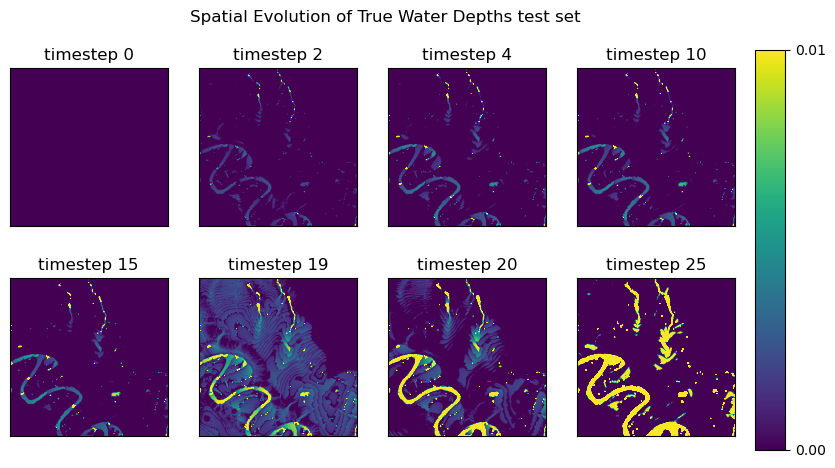
\includegraphics[width=0.8\linewidth, height=0.3\textheight]{Figures/Results/Final_Results/Best_Model_True_test_set}
	\caption[Spatial Evolution of True Water Depth for test set]{Spatial Evolution of True Water Depth for test set}
	\label{fig:SpatialTrue}
\end{figure}


\begin{figure}[tbph]
	\centering
	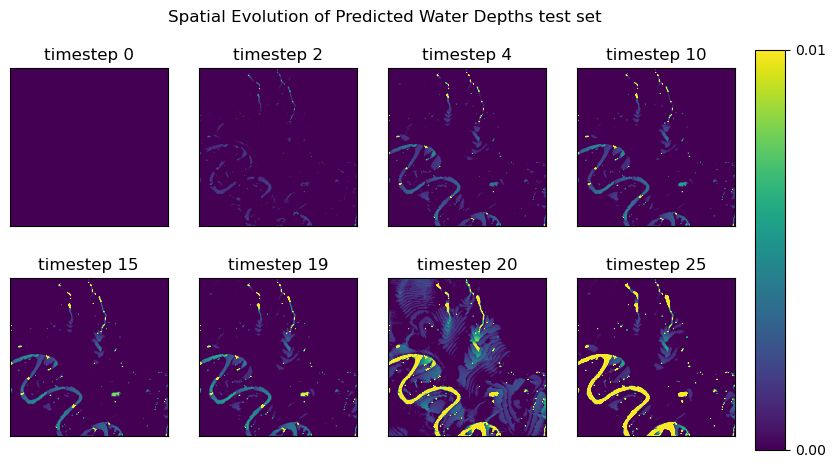
\includegraphics[width=0.8\linewidth, height=0.3\textheight]{Figures/Results/Final_Results/Best_Model_SS_SS_test_set}
	\caption[Spatial Single Time step Predictions]{Spatial Evolution for the Best Model Predicting single time steps}
	\label{fig:BMS-spatial}
\end{figure}


\begin{figure}[tbph]
	\centering
	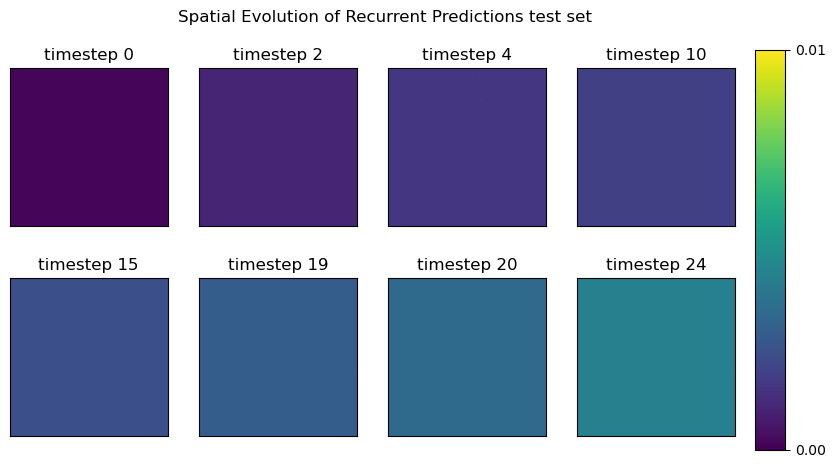
\includegraphics[width=0.8\linewidth, height=0.3\textheight]{Figures/Results/Final_Results/Best_SS_adjusted_weights(5,5)_spatial}
	\caption[Best Model with adjusted weights Spatial recurrent time step Predictions]{Spatial Evolution for the Best Model with adjusted weights (0.5, 0.5) Predicting Recurrent time steps}
	\label{fig:adjusted-spatial}
\end{figure}


\begin{figure}[tbph]
	\centering
	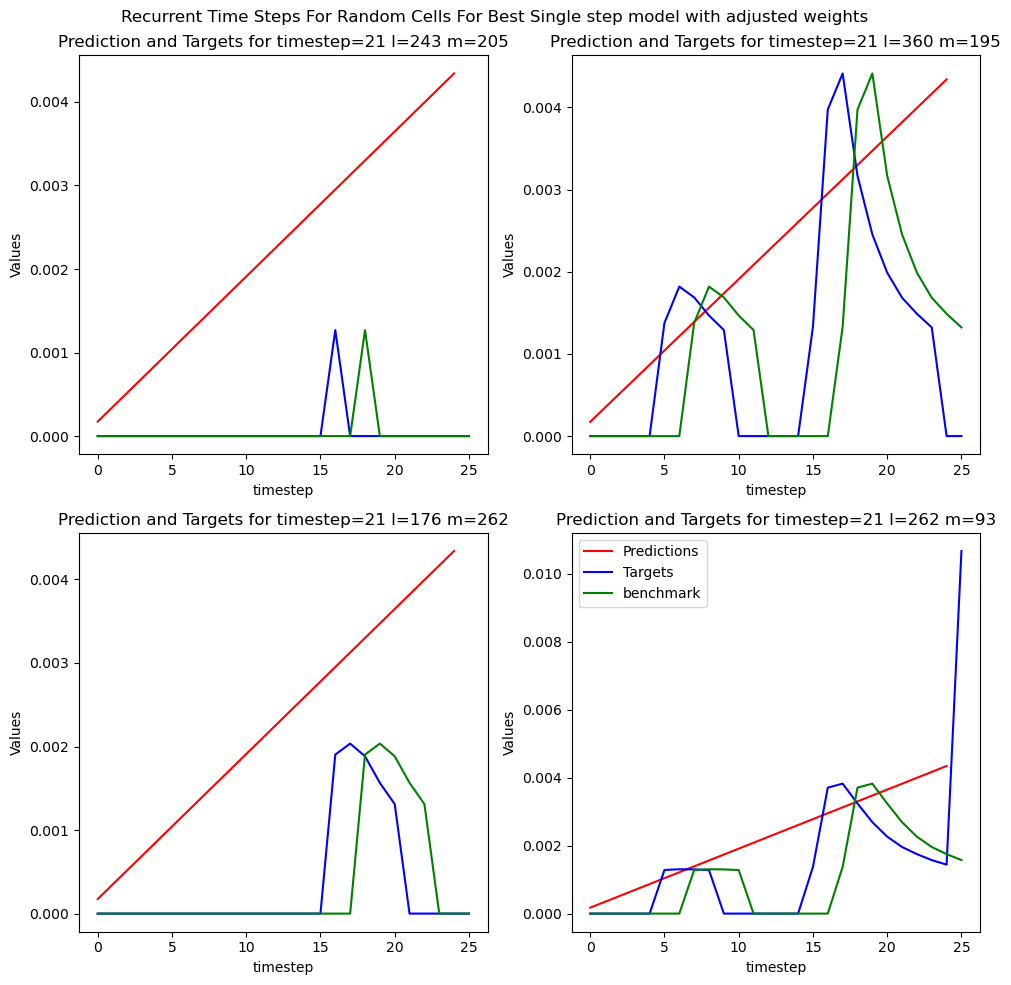
\includegraphics[width=0.8\linewidth, height=0.3\textheight]{Figures/Results/Final_Results/Best_SS_adjusted_weights(5,5)}
	\caption[Spatial Single Time step Predictions]{Spatial Evolution for the Best Model Predicting recurrent time steps but with adjusted weights (0.5, 0.5)}
	\label{fig:adjusted-recurrent-rc}
\end{figure}


\section{Limitations}
Although the vast majority of models outperformed the benchmark models and heuristic, they were unable to recurrently predict water depths across time points. Even single time step prediction was only predicting no change in water depth despite trying to account for this in the loss functions. There are many reasons for this which are outlined here,
\begin{enumerate}[align=left]
	\item[Normalization Strategy: ]  Only three normalization techniques were tested. This was a very difficult problem to tackle due to the range within features. Perhaps the way normalization was done, hindered the models ability to learn
	\item[Computational Limitations: ] Training data had to be sub sampled. Since time steps were 10 minute intervals and the DEM has a spatial resolution of 1 m, water is able to propagate many cells downstream in a single time step. Outside of the local neighborhood. When sub sampling is used, the model does not have access to this information. Which may have resulted in the models' being unable to learn correctly. This sub sampling technique also makes padding more of an issue. How is the model meant to know whether the data is outside a catchment area or whether it is just zero padding? It may be unable to determine this information. Or if a sub sample of data is upstream or downstream of another subsample. All of this is potentially useful information that the model may not have had access to due to computational constraints.
	\item[Loss Function and Metric: ] Perhaps the metric of evaluation could be improved. MAE error across the whole dataset may prioritize the model to predict no change as many of the cells are 0 from the simulated data. 
	\item[Unbalanced Data: ] The rainfall patterns are quite strange and most of the rainfall occurs in small time windows. Therefore most cells, at most time steps have 0 water depth. This means predicting 0 water depth results in a very low loss and the model easily recognizes this fact.
	\item[Single Time Step Prediction: ] A problem with this approach is not practically useful unless emergent properties like recurrent predictions are obtained which was not the case in this evaluation.
	\item[Evaluation: ] Metric had a fatal flaw and all testing done ultimately drove the model to predict no change in water depth. Even picking DEM 292 and the test set with 2 short spikes in rain fall (see DEM 292 in Fig. \ref{fig:4.4}). Future work should consider each training outcome in a case by case manner with far more careful evaluation to what the model is doing. A small experiment was performed in Section \ref{Extra} to highlight this.
\end{enumerate}

\section{Extras}
\label{Extra}
This section provides results from further testing that was done after the initial write up. Some optimistic results are presented after discovering the evaluation methods above were driving the model to predict zero change in water depth. The model used for this evaluation is as follows:

\begin{lstlisting}[language=Python]
	class SimpleCNN(tf.keras.Model):
		def __init__(self, model_config):
		super().__init__()
			self.config = model_config
			self.dmodel = tf.keras.Sequential([
			tf.keras.layers.Conv2D(80, 3, padding="same", activation=tf.nn.relu),
			tf.keras.layers.Conv2D(64, 1, activation=tf.nn.relu),
			tf.keras.layers.Conv2D(1, 1, activation=None)
			])
			self(tf.zeros([1, 3, 3, 3]))
		
		def call(self, x):
			dx = self.dmodel(x)
			f1, f2, f3 = tf.unstack(x, axis=-1)
			f1 =tf.expand_dims(f1, -1)
			return dx + f1
\end{lstlisting}
With model summary,

\begin{verbatim}
	Model: "simple_cnn_6"
	_________________________________________________________________
	Layer (type)                 Output Shape              Param #   
	=================================================================
	sequential_6 (Sequential)    (None, None, None, 1)     7489      
	=================================================================
	Total params: 7,489
	Trainable params: 7,489
	Non-trainable params: 0
	_________________________________________________________________
\end{verbatim}
We see that very few parameters are contained in this model. In this case, only the DEM was normalized and the rest were left un modified. Using the Manual MAE, but this time with zero weighting of 0.1 and non zero weighting of 0.9, we find much more promising results. See figures below.

\begin{figure}[tbph]
	\centering
	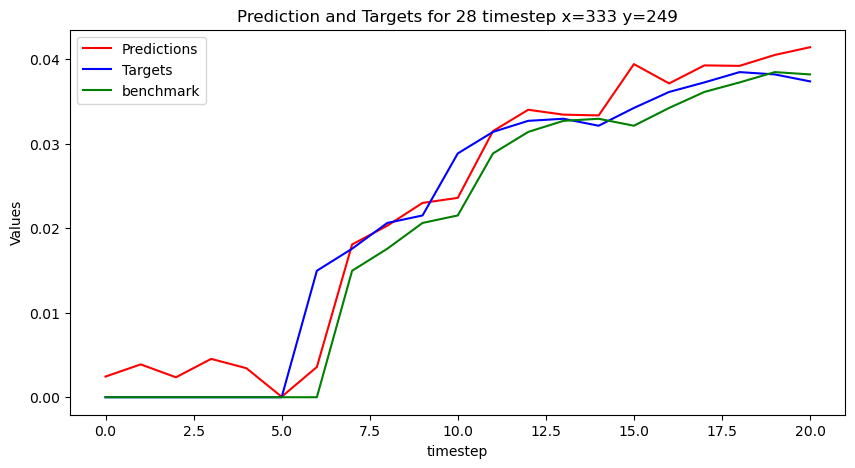
\includegraphics[width=0.8\linewidth, height=0.3\textheight]{Figures/Results/extra/extra_single_step}
	\caption[Extra Single Step prediction]{Single Step prediction versus heuristic and target for a random cell in the test dataset for DEM 26}
	\label{fig:extrasinglestep}
\end{figure}


\begin{figure}[tbph]
	\centering
	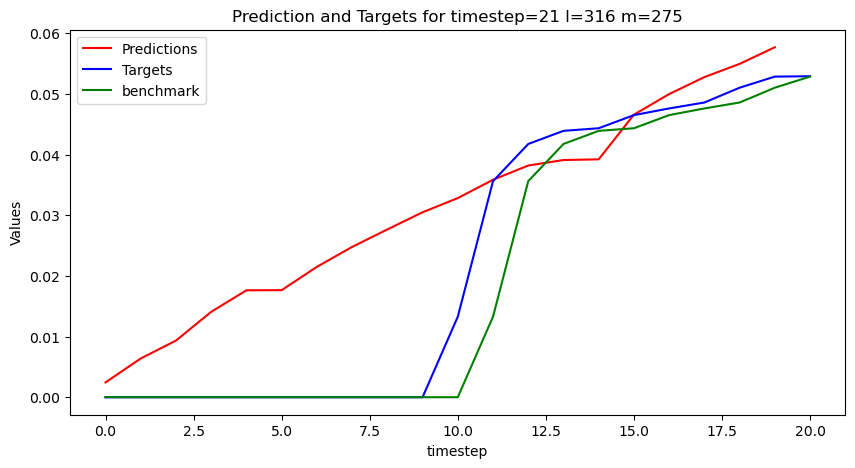
\includegraphics[width=0.8\linewidth, height=0.3\textheight]{Figures/Results/extra/extra_recurrent_step}
	\caption[Extra Recurrent Time Step Prediction]{Recurrent time step prediction versus heuristic and target for a random cell in test dataset DEM 26}
	\label{fig:extrarecurrentstep}
\end{figure}


\begin{figure}[tbph]
	\centering
	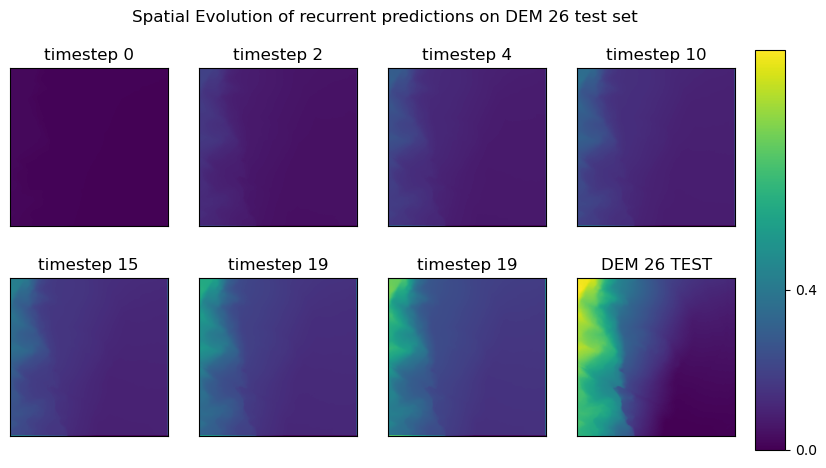
\includegraphics[width=0.8\linewidth, height=0.3\textheight]{Figures/Results/extra/Recurrent_Predictions_compare_dem}
	\caption[Recurrent Prediction vs DEM 26 map comparison]{Spatial evolution for the recurrent time step predictions. The final image is the DEM for dataset 26}
	\label{fig:recurrentpredictionscomparedem}
\end{figure}


\begin{figure}[tbph]
	\centering
	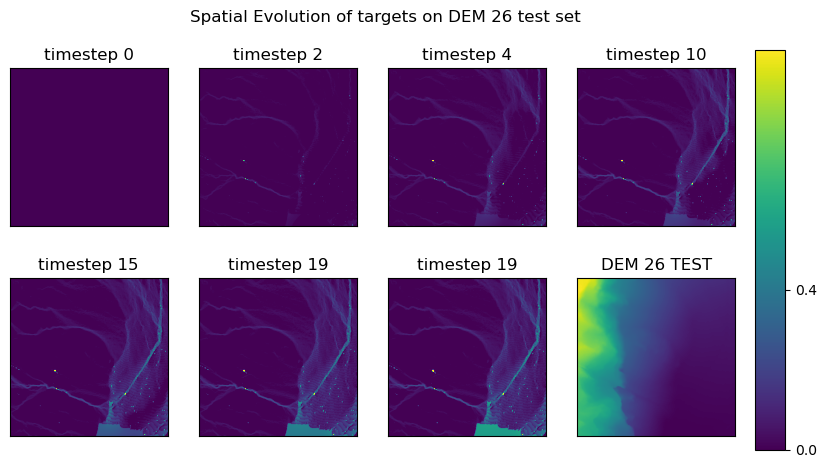
\includegraphics[width=0.8\linewidth, height=0.3\textheight]{Figures/Results/extra/Recurrent_targets_compare_dem}
	\caption[Targets for test dataset 26 comparison to DEM]{Spatial evolution for targets for test dataset DEM26. The final image is the DEM for dataset 26}
	\label{fig:recurrenttargetscomparedem}
\end{figure}


\begin{figure}[tbph]
	\centering
	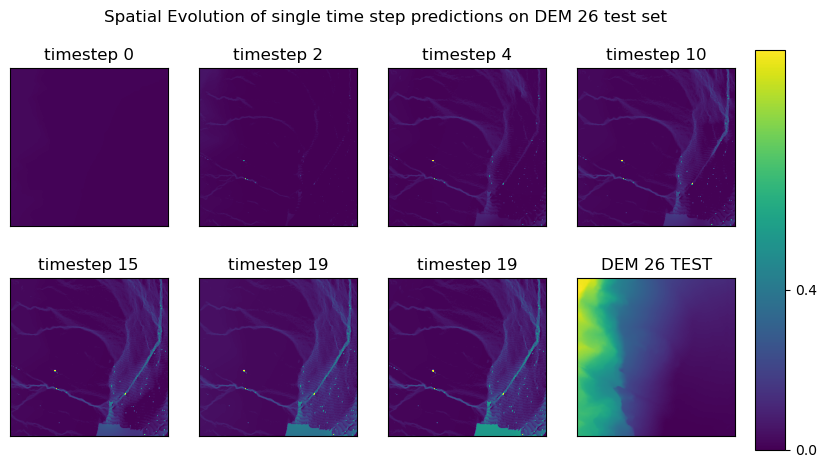
\includegraphics[width=0.8\linewidth, height=0.3\textheight]{Figures/Results/extra/SS_predictions_compare_dem}
	\caption[Spatial Evolution of Single Time Step predictions on test dataset DEM 26]{Spatial evolution for single time step predictions for test dataset DEM26. The final image is the DEM for dataset 26}
	\label{fig:sspredictionscomparedem}
\end{figure}


It is very  interesting to see that the recurrent predictions essentially are predicting the DEM map itself (see Fig \ref{fig:recurrentpredictionscomparedem}), or at  least its shape. This may be due to a bug of some kind but is interesting to see. Whereas the true values seem to be nothing like that (see Fig. \ref{fig:recurrenttargetscomparedem}). From Fig. \ref{fig:extrasinglestep} and \ref{fig:extrarecurrentstep} we see much more promising results than mentioned previously. These results were obtained using more training (50 epochs) and a learning rate of 0.001 with reduced learning rate as a call back. These results provide some hope that it is possible to model flooding behaviors with NCA. We can also see the similarities more visually between Fig \ref{fig:sspredictionscomparedem} and \ref{fig:recurrenttargetscomparedem}. Time step 19 shows a slight difference in water depth, where the model predicted a higher water depth for a single cell. The emergent properties seen in the recurrent time step predictions are also interesting, since the model was not explicitly trained to predict recurrently! The results for recurrent predictions are poor, however there are positive signs that it is possible but further evaluation and testing will be required. 
% Indicate the main file. Must go at the beginning of the file.
% !TEX root = ../main.tex

%----------------------------------------------------------------------------------------
% CHAPTER 6
%----------------------------------------------------------------------------------------
\chapter{Conclusion} % Main chapter title
\label{Chapter6} % For referencing the chapter elsewhere, use \ref{Chapter1}

\section{Conclusion}
\section{Outlook and future work}
% Indicate the main file. Must go at the beginning of the file.
% !TEX root = ../main.tex

%----------------------------------------------------------------------------------------
% CHAPTER 7
%----------------------------------------------------------------------------------------
\chapter{Conclusion} % Main chapter title
\label{Chapter7} % For referencing the chapter elsewhere, use \ref{Chapter1}

\section{Conclusion}
\section{Outlook and future work}

%----------------------------------------------------------------------------------------
% THESIS CONTENT - APPENDICES
%----------------------------------------------------------------------------------------
\appendix % Cue to tell LaTeX that the following "chapters" are Appendices

% Include the appendices of the thesis as separate files from the Appendices folder
% Uncomment the lines as you write the Appendices
% !TEX root = ../main.tex

%----------------------------------------------------------------------------------------
% APPENDIX A
%----------------------------------------------------------------------------------------

\chapter{Extra Notes on Deep Learning and materials} % Main appendix title

\label{AppendixA} % For referencing this appendix elsewhere, use \ref{AppendixA}

\section{Simple multilayer perceptron}

\begin{figure}[h]
	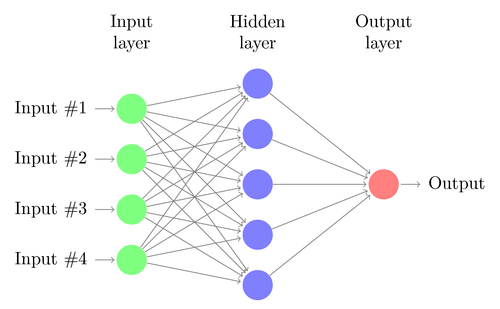
\includegraphics[width=0.75\textwidth]{../Figures/neural-network.png}
%	\centering
	\caption[An ANN]{A simple depiction of an artificial neural network} \url{https://texample.net/tikz/examples/neural-network/}
\label{fig:appendix-mlp}
\end{figure}

\begin{equation*}
	y =  \sigma\left(\sum WX + B\right)
\end{equation*}
Where
\begin{align*}
	y &  \text{ is the output or hidden layer} \\
	\sigma &  \text{is the activation function} \\
	X &  \text{ is the input vector} \\
	W &  \text{ is the weight vector} \\
	B &  \text{ Bias}
\end{align*}
Where Edges are weights and nodes are the sum of the weights *inputs + bias. An activation function like sigmoid or ReLu (which performs a kind of smooth mapping) is applied to this sum.

\section{Growing NCA}
\begin{figure}[h]
	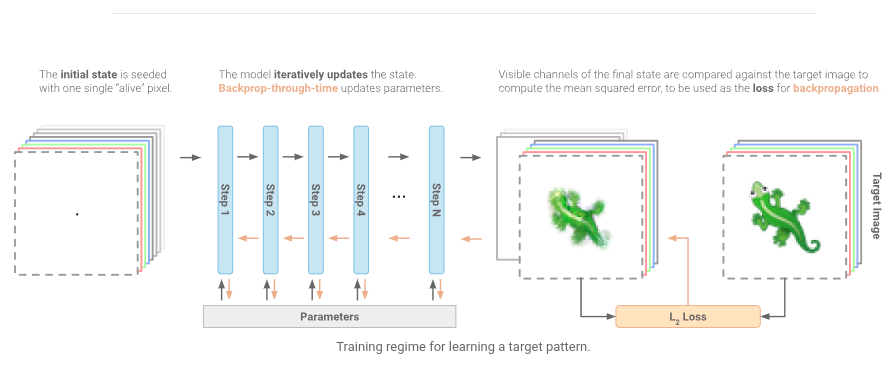
\includegraphics[width=1\textwidth]{../Figures/training_nca.png}
	\centering
	\caption[NCA-training]{How the model learns a target pattern. This image is taken directly the \citetitle{growing_nca} paper \cite{growing_nca}} 
	\label{fig:appendix-nca}
	\url{https://distill.pub/2020/growing-ca/}
\end{figure}
%\section{How can I add a Figure in the Appendix?}
%
%You can refer to a figure in the Appendix (like \ref{fig:appendix-figure}) and it will show up as expected.
%
%\begin{figure}
%\includegraphics[width=0.25\textwidth]{../Figures/Bart_Simpson.png}
%\centering
%\caption[A random appendix figure]{Bart Simpson. (2023, May 17). In Wikipedia. \url{https://en.wikipedia.org/wiki/Bart_Simpson}}
%\label{fig:appendix-figure}
%\end{figure}

% !TEX root = ../main.tex

%----------------------------------------------------------------------------------------
% APPENDIX C
%----------------------------------------------------------------------------------------

\chapter{Building Intuition About NCA} % Main appendix title

\label{AppendixB} % For referencing this appendix elsewhere, use \ref{AppendixB}

Based on the amazing work of \citeauthor{growing_nca} and his associated tutorials \footnote{A link to his youtube channel \href{https://www.youtube.com/@zzznah}{here}} , I implemented a simplified version of this NCA in Tensorflow. The first attempt was just copying the code and playing with the notebook available \href{https://colab.research.google.com/github/google-research/self-organising-systems/blob/master/notebooks/growing_ca.ipynb}{here}. Next was simplifying the model to point I could understand the code. It turns out that a lot of the work that went into this paper was creating an incredibly robust model that was invariant to many factors, such as rotation, regrowth, and persistence. All of which I didn't really need for my purposes. And once I had a grasp of the basic concepts I could expand the model / training as needed.

Some things I did not implement from the paper:
\begin{itemize}
	\item Damaging the model to train for regrowth
	\item Playing around with the fire rate as 0.5 seemed to work best based on the paper anyways
	\item Creating a circle mask around the image such that it doesn't rely on edges to grow certain features (or in some cases the whole image)
\end{itemize}

One method I implemented from the original paper was the pooling section. 
\begin{lstlisting}[language=Python]
class Pooling:
	def __init__(self, n_channels=16, pool_size=1024, size=(40,40),  padding_size=16, sample_size=8):
		self.pool_size = pool_size
		self.n_channels = n_channels
		self.sample_size = sample_size
		self.size = size
		seed = Pooling.make_seed(size[0]+padding_size, size[1]+padding_size, self.n_channels)
		self.the_pool = seed.repeat(self.pool_size, axis=0)
	
	def get_sample(self):
		inds = np.random.choice(self.pool_size, self.sample_size, False)
		batch = self.the_pool[inds]
		return inds, batch
	
	def commit(self, inds, outputs):
		self.the_pool[inds] = outputs
		   
\end{lstlisting}
This is just a way to artificially increase the amount of iterations the model performs to make sure that once the image has been accurately grown, the image remains after an arbitrary amount of time-steps. It does this by sampling final grown images from training and uses this as the initial configuration of the model. So if during training, you start from a seed configuration of a single black pixel in the center of the blank image, and allow it to grow to grow for example 50 time steps until it produces an image, then during the next iteration of training, the initial configuration will be that image and needs to remain that image for 50 time-steps. Essentially artificially increasing the time steps from 50 to 100 without having to perform back-propagation over 100 time-steps.

There were some issues with this method though. If you don't have a sufficiently large enough pool then the pool might get clogged up with terrible, failed images that are essentially just noise. it is better to use this at later stages of training when it isn't growing randomly.
% !TEX root = ../main.tex

%----------------------------------------------------------------------------------------
% APPENDIX C
%----------------------------------------------------------------------------------------

\chapter{Review of \citetitle{Ghimire} by \citeauthor{Ghimire}} % Main appendix title

\label{AppendixC} % For referencing this appendix elsewhere, use \ref{AppendixC}

This appendix was part of my work for track module 1 and may be helpful in understanding the updated paper.
\section{CA Approach}
There are a few problems with conventional flood modeling techniques. 1D models give us limited information about flow dynamics and 2D models are extremely computationally taxing, which limits their use. Cellular automata (CA) could be implemented to remedy this problem by reducing the computational time and cost to run these models. The focus of this review will be primarily on the CA created by \cite{Ghimire} as the paper is very well laid-out and the CA used is well defined, albeit, complex. This CA uses regular grid cells as a discrete space for the CA setup and applies generic rules to local neighbourhood cells to simulate the progression of pluvial floods.

\section*{CA Formulation by Ghimire, et al}

This model consists of five essential features of a true cellular automation: discrete space; neighbourhood (NH); cell state; discrete time step; transition rule.
The square grid digital elevation model (DEM) provides the discrete space for the CA set up. A DEM is just a representation of the bare ground (bare earth) topographic surface of the Earth which excludes trees, buildings, and any other surface objects \cite{DEM}. The NH used for this model consists of the central cell itself and its four cardinal adjacent cells (five cells in total). This is known as the von Neumann type NH. The Moore NH, consisting of eight surrounding cells and the central cell similar to the NH in John Conway’s Game of Life, is an alternative. 
Precipitation occurs over the whole area of the terrain being considered. Movement of the water is mainly driven by the slopes between cells and limited by the transferrable volume and the hydraulic equations. The transferrable volume is the minimum of the total volume within the giving cell and the space available in the receiving cells. The transferrable volume is the minimum of the total volume within the giving cell and the space available in the receiving cells. Manning’s equation and the critical flow equation are applied to restrict the flow velocity. The assumption here is that water can only flow from one cell to its local NH, according to the hydraulic gradients in one computing time step. 
In the calculation the NH cells are ranked according to the water level, as 1 for the cell with the lowest level and 5 for the highest one, to determine the direction of flow between cells. Only the outflow fluxes (Flux as flow rate per unit area) from the central cell to its neighbours with lower ranks are calculated. Any inflow to the cells under consideration is eventually calculated as the outflow from its neighbor that has a higher water level on the opposite of the cell interface.
The fluxes through the interfaces of the central cell are determined by the states of NH cells in previous time steps and stored as intermediate buffers for updating the states of cells. The states of flood depths of all cells are updated simultaneously when all interface fluxes are determined.

\subsection*{Main Algorithm:}
Program start
\begin{enumerate}
	\item Initialize variables –depth, water surface elevation, input(terrain, rainfall)
	\item Start time loop\{
	\item Add precipitation depth directly to the water depth on the cells
	\item Computation starts in the local NH \{
	\begin{enumerate}
		\item Ascending cell rankings based on the water surface elevations
		\item Layer-wise claculation of outflows from central cell
		\item Distribution of layer-wise fluxes within the NH
		\item Calculate the cell interfacial velocities
	\end{enumerate}
	\item End of local NH loop \}
	\item Determine time step $\Delta$t required for the distriibutions appiled
	\item Update simulation time: t = t + $\Delta$t
	\item Update the states (depths, water surface elevation) for the new time step
	\item Apply boundary conditions to suit the flow conditions
	\item Data outputs for visualization and analysis
	\item Repeat until the end of simulation time
	\item End of time loop \}
\end{enumerate}
Program end

\subsection*{Outflow Flux Calculation}
The calculation process starts with cell ranking, based on the water surface elevation in the local NH with five discrete states of cell ranks \{r=1, 2, 3, 4, 5\}. This is the height of each cell. Space between the water levels (water levels added on top of the height) of the cells are divided into four layers. Li ¬ is the free space between the water levels of cells ranked i and i + 1 that can accommodate the water volume from cells with higher ranks. If the rank of the central cell is r¬c (e.g. rank 3) there can be at most rc -1 number of cells receiving water as flux (because the central cell obviously can’t receive water from itself) through the NH cell boundaries, if enough water is available in the central cell. Outflow volume to the layer i can be given by the following formula that is applied locally for each cell considered: 
\begin{equation} \label{eq:1}
	\Large\Delta{V}_{i} = \text{min}\Big\{V_{c} - \sum_{k=1}^{i-1} \Delta{V}_{k}, \Delta{WL}_{i}\sum_{k=1}^{i}A_{k}\Big\}
\end{equation}
Where $V_{c}$ is the water volume of the central cell in the previous time step; $\Delta$ $V_{k}$ is the volume distributed to layer $k$, $\sum_{k=1}^{i-1}$$\Delta{V}_{k}$ total volume has has been distributed to layers 1 to i-1; $V_{c}$ - $\sum_{k=1}^{i-1}$$\Delta{V}_{k}$ represents the remaining volume available for distributing to layer i  after filling i-1 layers. $\Delta{WL}_{i}$ is the water level difference between cells ranked i and i+1;  $\sum_{k=1}^{i}$$\Delta{A}_{k}$ is the total surface area of layer i; $\Delta{WL}_{i}$  $\sum_{k=1}^{i}$$\Delta{A}_{k}$ is the available space for storage in layer i. For the layer adjacent to the central cell, an additional term
\begin{displaymath}
	\Large \sum_{k=1}^{i} A_{k}/A_{c} + \sum_{k=1}^{i} A_{k}\Big(V_{c} - \sum_{k=1}^{i-1} \Delta{V}_{k} \Big)
\end{displaymath}
is applied to limit $\Delta{V_{i}}$, which assumes that the water levels for all cells will reach an equivalent level. Thus, a cell with rank r receives water only from cells with higher ranks and the water received is added on top of its own water level. Thus, the total outflow flux from the central cell to a neighbouring cell ranked i is calculated as:
\begin{equation} \label{eq:2}
	\Large F_{i} = \sum_{k=i}^{r_{c} - 1}\frac{\Delta{V_{k}}}{k}
\end{equation}
For a regular grid, the areas of the central cell, $A_{c}$ and the neighboring cells, $A_{k}$ are constant over the domain. However, the methodology is applicable to different grid settings. Therefore, a cell containing buildings that do not allow water to flow in can be described using a variable cell area to reflect the reduced space occupied by buildings.

\subsection*{Depth updating}
A very important step in the CA approach is the execution of the state transition rule. In the resent CA calculations, the global continuous state is the flow depth in a grid cell, which is updated for every new time step. This is done by algebraically summing the water depth from all its four neighbours. The following transition rule is used to update the flow depth:

\begin{equation} \label{eq:3}
	\Large d^{t+\Delta{t}} = d^{t} + \theta \frac{\sum F}{A}
\end{equation}
Where $\theta$ is a non-dimensional flow relaxation parameter that can take values between 0 and 1, F is the total volume transferred to the cell under consideration as calculated from Equation $\ref{eq:2}$ and A is the cell area. The purpose of the relaxation parameter is to damp oscillations that would appear otherwise. The effect of the relaxation parameter does not impart any effect on mass conservation rather it makes the flow smooth and gradual. The values of $\theta$ are determined by numerical experiments and calibration.

\subsection*{Time-Step Calculation}

For most 2D hydraulic modelling, higher resolution DEM data are being used, the required time steps will be shorter to ensure the stability of model computations, which often leads to large computational burden, such that many studies have been focused on reducing the computational time of simulations. The time increment, determined as the largest that satisfies the stability criteria anywhere in the whole domain, implies that for most of the cells only a fraction of the locally allowable time steps is used to integrate the solution in time. This represents a waste of computational effort and limits the use of the method. A spatially varying time step can increase solution accuracy and reduce computer run time. In this implementation we use maximum permissible velocity which ensures the minimum time steps required to distribute the applied flux. The interfacial velocity v* is determined based on the flux transferred through a cell boundary given by:

\begin{equation} \label {eq:4}
	\Large v^{*} = \frac{F}{d^{*}\Delta{x}\Delta{t}}
\end{equation}
Where, $ d*$ is the water depth of flow available at the interface, which is the difference between higher water level and higher ground elevation of the central cell and its neighbour cell to the interface

\begin{equation} \label{eq:5}
	\Large d* = \text{max} \{WL_{C}, WL_{N}\} - \text{max}\{z_{C}, z_{N}\}
\end{equation}

Where, $WL$ and $z$ are the water levels and ground elevation respectively and the subscripts $C$ and $N$ represent central and neighbouring cells repectively
To prevent the velocity from over shooting, a cap on the localallowable velocity is applied as given by Equation \ref{eq:6} based on the Manning's formula and critical flow condition as:
\begin{equation} \label{eq:6}
	\Large v = \text{min}\{\frac{1}{n}R^{\frac{2}{3}}S^{\frac{1}{2}}, \sqrt{gd}\}
\end{equation}
where, the hydraulic radius R is taken to be equal to the water depth $d$ and $S$ is the slope of water surface elevation and is always positive for outflow calculation. If $v$ is less than $v*$, the interfacial flux $F$ is recalculated by replacing $v*$ with $v$ in Equation \ref{eq:4}
The global time step is then calculated based on the global maximum velocity to satisfy the conventional CFL criteria. Therefore, each time the state transition rule is applied, the global time step is updated using maximum velocity calculated from all cell interfaces, as given by:
\begin{equation} \label{eq:7}
	\Large \Delta{t} = \frac{\Delta{x}}{\text{max}\{v_{j}\}}
\end{equation}
Where $v_{j}$ is the velocity calculated for the jth cell interface for the entire domain.
% from https://www.zhaw.ch/en/lsfm/study/studiweb/master-ls/masters-thesis/
%

\include{Appendices/DeclarationOfOriginalityZHAW} 


%----------------------------------------------------------------------------------------
% BIBLIOGRAPHY
% I need to compile using biber instead of bibTex...
%----------------------------------------------------------------------------------------
\printbibliography[heading=bibintoc]

%----------------------------------------------------------------------------------------

\end{document}  
